%definira klasu dokumenta 
\documentclass[12pt]{report} 

%prostor izmedu naredbi \documentclass i \begin{document} se zove uvod. U njemu se nalaze naredbe koje se odnose na cijeli dokument

%osnovni LaTex ne može riješiti sve probleme, pa se koriste različiti paketi koji olakšavaju izradu željenog dokumenta
\usepackage[croatian]{babel} 
\usepackage{amssymb}
\usepackage{amsmath}
\usepackage{txfonts}
\usepackage{mathdots}
\usepackage{titlesec}
\usepackage{array}
\usepackage{lastpage}
\usepackage{etoolbox}
\usepackage{longtable, tabu}
\usepackage{color, colortbl}
\usepackage{adjustbox}
\usepackage{geometry}
\usepackage[classicReIm]{kpfonts}
\usepackage{hyperref}
\usepackage{fancyhdr}
\usepackage{comment}

\usepackage{float}
\usepackage{setspace}
\restylefloat{table}


\patchcmd{\chapter}{\thispagestyle{plain}}{\thispagestyle{fancy}}{}{} %redefiniranje stila stranice u paketu fancyhdr

%oblik naslova poglavlja
\titleformat{\chapter}{\normalfont\huge\bfseries}{\thechapter.}{20pt}{\Huge}
\titlespacing{\chapter}{0pt}{0pt}{40pt}


\linespread{1.3} %razmak između redaka

\geometry{a4paper, left=1in, top=1in,}  %oblik stranice

\hypersetup{ colorlinks, citecolor=black, filecolor=black, linkcolor=black,	urlcolor=black }   %izgled poveznice


%prored smanjen između redaka u nabrajanjima i popisima
\newenvironment{packed_enum}{
	\begin{enumerate}
		\setlength{\itemsep}{0pt}
		\setlength{\parskip}{0pt}
		\setlength{\parsep}{0pt}
	}{\end{enumerate}}

\newenvironment{packed_item}{
	\begin{itemize}
		\setlength{\itemsep}{0pt}
		\setlength{\parskip}{0pt}
		\setlength{\parsep}{0pt}
	}{\end{itemize}}


%boja za privatni i udaljeni kljuc u tablicama
\definecolor{LightBlue}{rgb}{0.9,0.9,1}
\definecolor{LightGreen}{rgb}{0.9,1,0.9}


%podesavanje zaglavlja i podnožja

\pagestyle{fancy}
\lhead{Programsko inženjerstvo}
\rhead{Terminko}
\lfoot{Janezi}
\cfoot{stranica \thepage/\pageref{LastPage}}
\rfoot{\today}
\renewcommand{\headrulewidth}{0.2pt}
\renewcommand{\footrulewidth}{0.2pt}


\begin{document} 
	
	
	
	\begin{titlepage}
		\begin{center}
			\vspace*{\stretch{1.0}} %u kombinaciji s ostalim \vspace naredbama definira razmak između redaka teksta
			\LARGE Programsko inženjerstvo\\
			\large Ak. god. 2020./2021.\\
			
			\vspace*{\stretch{3.0}}
			
			\huge Terminko za praonicu rublja\\
			\Large Dokumentacija, Rev. \textit {2}\\
			
			\vspace*{\stretch{12.0}}
			\normalsize
			Grupa: \textit Janezi\\
			Voditelj: \textit {Jan Grgić}\\
			
			
			\vspace*{\stretch{1.0}}
			Datum predaje: \textit{13. studenoga 2020.}\\
	
			\vspace*{\stretch{4.0}}
			
			Nastavnik: \textit {Izv. Prof. Dr. Sc. Vlado Sruk}\\
		
		\end{center}

	
	\end{titlepage}

	
	\tableofcontents

	\chapter{Dnevnik promjena dokumentacije}
		
		\textbf{\textit{Kontinuirano osvježavanje}}\\
				
		
		\begin{longtabu} to \textwidth {|X[2, l]|X[13, l]|X[5, l]|X[4, l]|}
			\hline \multicolumn{1}{|l|}{\textbf{Rev.}}	& \multicolumn{1}{l|}{\textbf{Opis promjene/dodatka}} & \multicolumn{1}{|l|}{\textbf{Autori}} & \multicolumn{1}{l|}{\textbf{Datum}} \\[3pt] \hline
			\endfirsthead
			
			\hline \multicolumn{1}{|l|}{\textbf{Rev.}}	& \multicolumn{1}{l|}{\textbf{Opis promjene/dodatka}} & \multicolumn{1}{|l|}{\textbf{Autori}} & \multicolumn{1}{l|}{\textbf{Datum}} \\[3pt] \hline
			\endhead
			
			\hline 
			\endlastfoot
			
			0.1 & Napravljen predložak.	& D. Grgić & 20.10.2020. 		\\[3pt] \hline 
			0.2	& Promijenjeni dijelovi predloška. & J. Grgić & 21.10.2020. 	\\[3pt] \hline 
			0.3 & Prepisan opis projektnog zadatka iz word dokumenta koji je sastavljen ranije radi prijave vlastite teme. & J. Grgić & 22.10.2020. 		\\[3pt] \hline
			0.4 & Dodani dionici u poglavlju 3, navedeni aktori i funkcionalni zahtjevi za neregistrirane/neprijavljene korisnike. Napisani obrasci uporabe za neregistrirane/neprijavljene korisnike.	& J. Grgić & 23.10.2020. 		\\[3pt]
		    \hline 
		    0.5 & Uređen dnevnik sastajanja i podjela poslova u grupi.	& J. Grgić & 23.10.2020. 		\\[3pt] \hline
		    0.6 & Dodani funkcionalni zahtjevi za Administratora. & I. Joskić & 23.10.2020. \\[3pt] \hline
			0.7 & Dodani funkcionalni zahtjevi za Korisnika.  & B. Spiegl & 23.10.2020. \\[3pt] \hline
		    0.8 & Dodani obrasci uporabe za Administratora. & I. Joskić & 23.10.2020. \\[3pt] \hline
		    0.9 & Navedeni funkcionalni zahtjevi za Zaposlenika. & M. Dragošević & 24.10.2020. \\[3pt] \hline
		    0.10 & Dodani obrasci uporabe za Zaposlenika. & M. Dragošević & 24.10.2020. \\[3pt] \hline
		    0.11 & Dodani opisi tablica u bazi podataka. & D. Šmigovec & 25.10.2020. \\[3pt] \hline
		    0.12 & Promjena baze podataka. & D. Šmigovec & 25.10.2020. \\[3pt] \hline
			0.13 & Dodan 3. sastanak u dnevnik sastajanja & J. Grgić & 26.10.2020. \\[3pt] \hline
			0.14 & Dodani ostali zahtjevi. & D. Grgić & 26.10.2020. \\[3pt] \hline
			0.15 & Dodano još obrazaca uporabe za Administratora. & I. Joskić & 26.10.2020. \\[3pt] \hline
			0.16 & Dodano još obrazaca uporabe za Registriranog korisnika i modificirani funkcionalni zahtjevi zajedno sa odgovarajućim obrascima upotrebe. & B. Spiegl & 29.10.2020. \\[3pt] \hline
			0.17 & Dodan obrazac uporabe za plaćanje i prvi dijagram obrasca uporabe za registrirane i neregistrirane korisnike. & J. Grgić & 31.10.2020. \\[3pt] \hline
			0.18 & Dodani sekvencijski dijagrami za UC1 i UC11. & I. Joskić & 31.10.2020. \\[3pt] \hline
			0.19 & Dodani sekvencijski dijagrami za UC3 i UC4. & D. Šmigovec & 31.10.2020. \\[3pt] \hline
			0.20 & Dodani opisi za sekvencijske dijagrame \ref{fig:skvDReg} i \ref{fig:skvDOglas}. & I. Joskić & 1.11.2020. \\[3pt] \hline
			
		\end{longtabu}
	
	
		\textit{Moraju postojati glavne revizije dokumenata 1.0 i 2.0 na kraju prvog i drugog ciklusa. Između tih revizija mogu postojati manje revizije već prema tome kako se dokument bude nadopunjavao. Očekuje se da nakon svake značajnije promjene (dodatka, izmjene, uklanjanja dijelova teksta i popratnih grafičkih sadržaja) dokumenta se to zabilježi kao revizija. Npr., revizije unutar prvog ciklusa će imati oznake 0.1, 0.2, …, 0.9, 0.10, 0.11.. sve do konačne revizije prvog ciklusa 1.0. U drugom ciklusu se nastavlja s revizijama 1.1, 1.2, itd.}
	\chapter{Opis projektnog zadatka}
		
		\section{Opis problema i motivacija}
		
			{Jedan je od glavnih problema života u studentskom domu pranje rublja. Studenti smješteni u domove
			moraju paziti na raspored pranja više nego na rokove za prijavu ispita, jer što im znači prijavljen ispit ako
			na njega nemaju u čemu doći. Motivacija za izradu ove web aplikacije leži u nepraktičnom sustavu
			rezerviranja termina pranja odjeće. Često se zna dogoditi da se student dođe upisati, ali naiđe na
			zatvorena vrata zbog pauza koje su stalno u drugo vrijeme ili nađe kompletno popunjen kalendar te ne
			može oprati veš. Želimo da se to iskustvo olakša studentima, ali i zaposlenicima praonice. Na ovaj bi se
			način mogli puno jednostavnije rezervirati, ali i otkazati termini za pranje koji bi se onda lako popunili te
			bi se studenti mogli puno bolje organizirati pa čak i upisati za termin koji je netom otkazan.
			Moderniziralo bi se i plaćanje te penaliziralo često otkazivanje dragocjenih termina.}
		
		\section{Postojeća slična rješenja}
		
			{Istraživanjem tržišta, zaključili smo da postoji nekoliko aplikacija koje se bave navedenim problemima.
			Jedna je od aplikacija koju smo uspjeli pronaći, a da je slična onome što želimo proizvesti slijedeća:
			\url{https://play.google.com/store/apps/details?id=net.celestialdata.ujlaundry&hl=en_US} (Slika  \ref{fig:ujlaundry}). Ta je aplikacija
			razvijena za praonicu na University of Jamestown-u. Dakako, razlika je u tome što je ovo isključivo
			mobilna aplikacija (postoje verzije za Android I IOS), a mi bismo napravili responzivnu web aplikaciju lako
			dostupnu svima s bilo kojeg uređaja koji ima pristup internetskoj mreži. Također, imamo I neke dodatne
			funkcionalnosti koje su navedene u usporedbi sa slijedećom aplikacijom (posudba košare, recenzije
			radnika, objava slika, oglasi za posao... ).}
		
			\begin{figure}[H]
				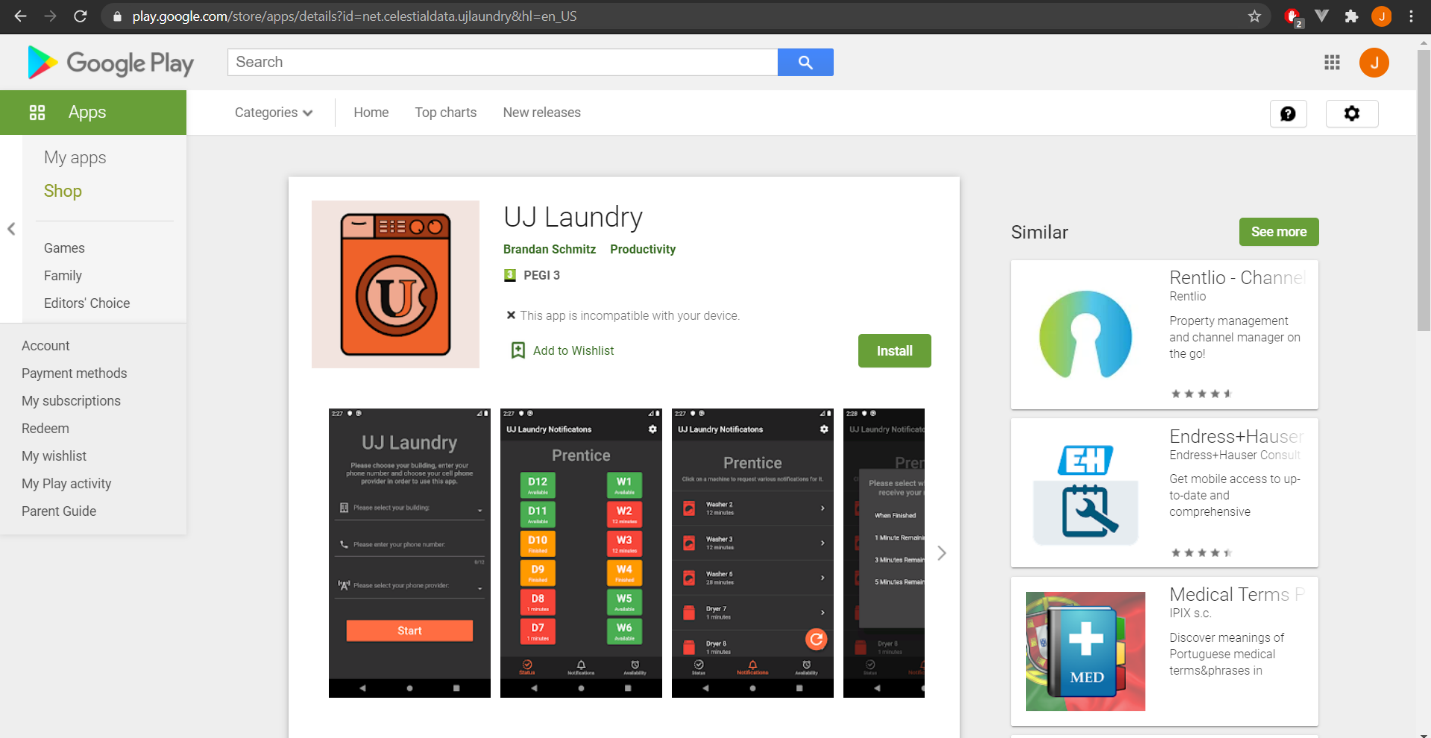
\includegraphics[width=.9\linewidth]{slike/UJLAUNDRY.PNG}
				\caption{Slika aplikacije "UJLAUNDRY"}
				\label{fig:ujlaundry}
			\end{figure}
		
			{Također, pronašli smo I slijedeću aplikaciju Nizozemskog porijekla: \url{https://www.duwo.nl/en/irent/residence-matters/washing-machine-with-a-qr-code} (Slika  \ref{fig:duwo}). Ta je aplikacija po glavnoj funkcionalnosti 
			poprilično slična našoj (web aplikacija koja omogućuje online rezervaciju termina i plaćanje preko
			interneta. Razlike su u tome što bi naša aplikacija bila prilagođenija studentskim domovima. Nudila bi
			funkcionalnost označavanja osobe koja je posudila košaru, recenzije radnika u praoni (što druge
			aplikacije nemaju jer su većinom vešeraju samoposlužni, duk je u domu zaposlen radnik), mogućnost
			objavljivanja slika izgubljenih stvari, mogućnost administratora da objavi oglas za posao u praoni, te
			mogućnost promijene radnog vremena, odnosno vremena pauzi na dnevnoj bazi. Također, ta aplikacija
			nema mogućnost slanja obavijesti na mail (npr. 1h prije početka termina).}
		
			\begin{figure}[H]
				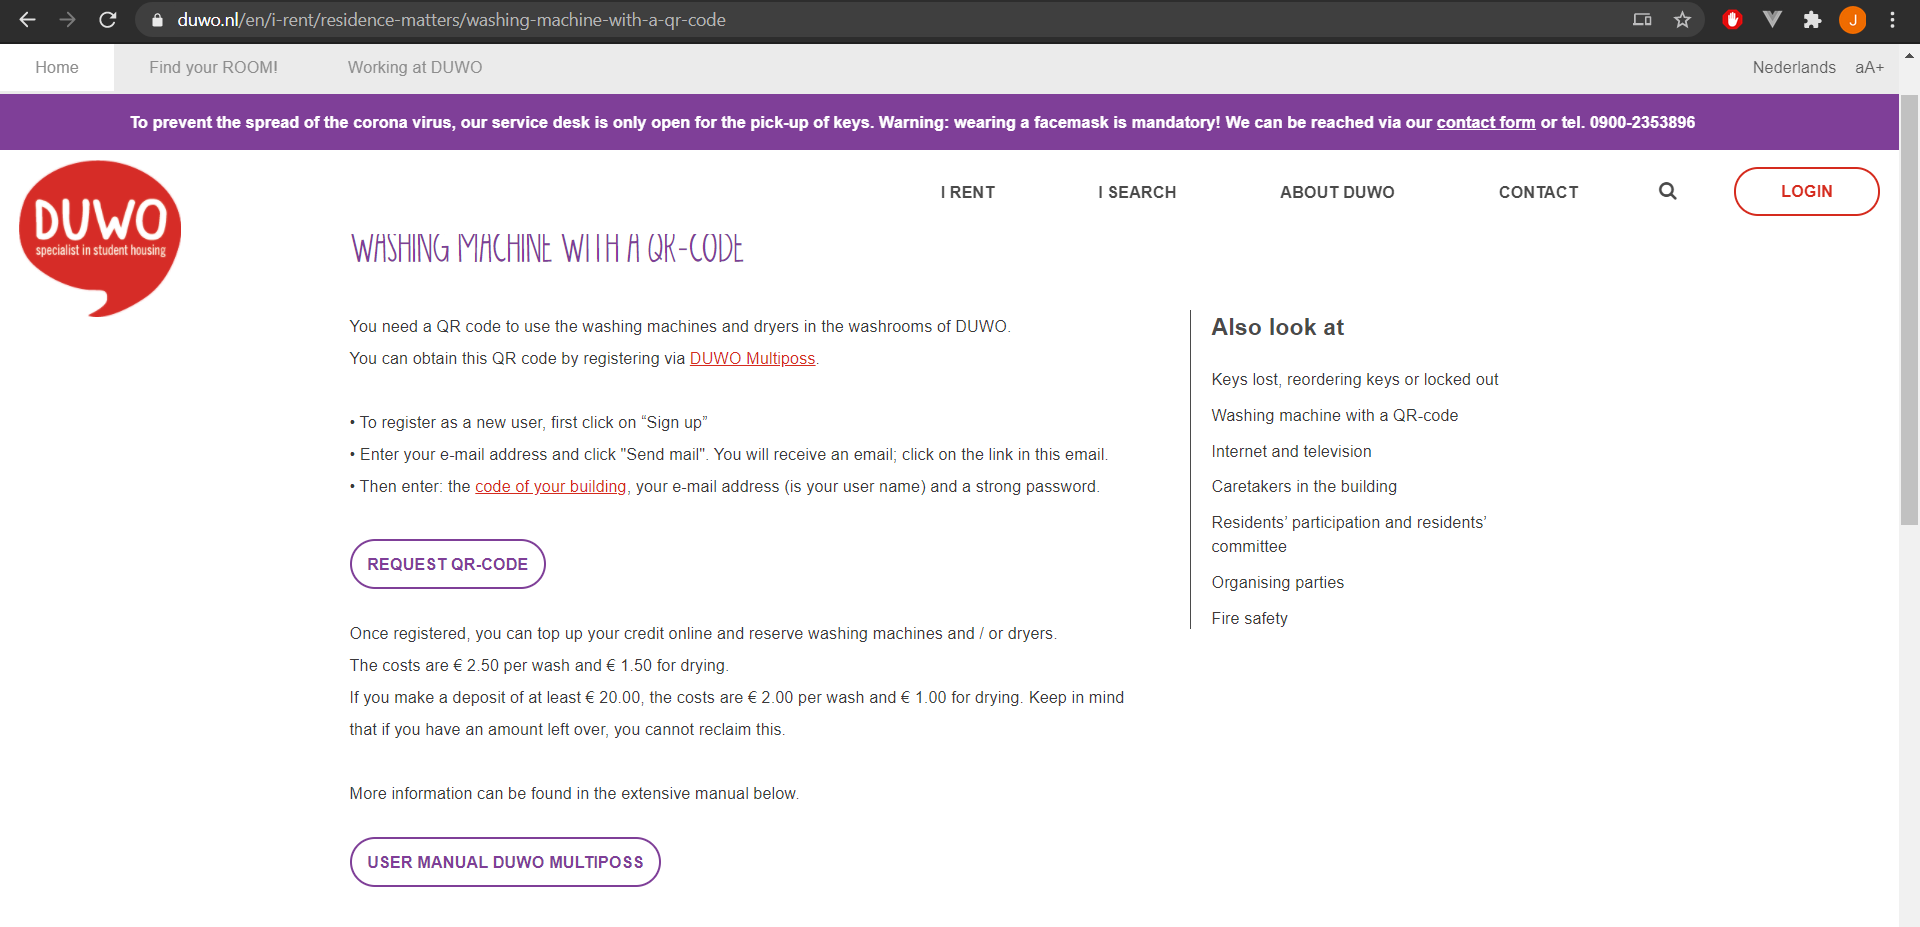
\includegraphics[width=.9\linewidth]{slike/DUWO.PNG}
				\caption{Slika aplikacije "Washing machine with a QR code"}
				\label{fig:duwo}
			\end{figure}
		
			{Treća pak stranica koju smo pronašli dolazi iz Norveške (Slika  \ref{fig:sit}). Sličnih je funkcionalnosti kao i prethodno
			navedena Nizozemska aplikacija, osim što ima dodatnu funkcionalnost, a to je slanje sms poruka za
			obavijesti (razlika u odnosu na našu je što bi mi slali na mail). Što se razlika tiče, slične su kao i u gore
			navedenom primjeru, uz razliku u tome što ova aplikacija, kao i naša, implementira slanje obavijesti
			korisnicima. }
		
			\begin{figure}[H]
				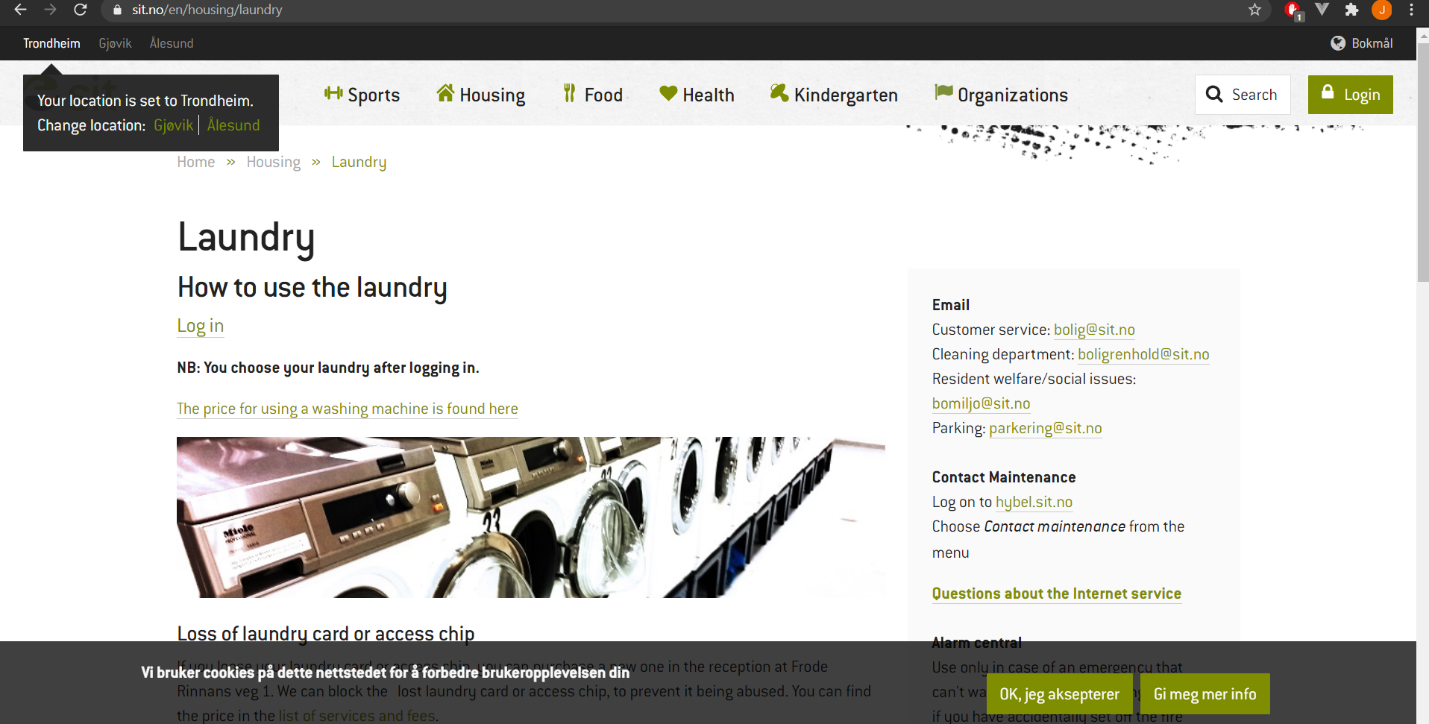
\includegraphics[width=.9\linewidth]{slike/SIT.PNG}
				\caption{Slika aplikacije za rezervaciju termina iz Norveške}
				\label{fig:sit}
			\end{figure}
		
			{Postoji i još nekoliko aplikacija sličnoga karaktera, no naveli smo 3 najpopularnije. Većina ostalih
			aplikacija dijele slične razlike u usporedbi s našom kao i gore navedene pa bi bilo redundantno navoditi
			ih.}
			
		\section{Potencijalno zainteresirani korisnici}
			
			{Za ovaj projekt očekujemo da će najveći interes pokazati studentski domovi s obzirom da je cilj projekta
			olakšavanje poslovanja već postojećih praonica veša u sklopu domova. No unatoč prvobitnom
			usmjerenju projekta prema studentskim domovima, smatramo da je ovakvo rješenje također opće
			primjenjivo i na ostale javne praonice jer primjenom ovakvog rješenja sa mogućnošću online rezervacije
			termina korisnik ne bi morao riskirati dolazak u punu praonicu te bi mogao izbjeći nepotrebno čekanje.
			Projekt bi također bilo moguće uvesti u ostale ustanove koje nude mogućnosti pranja veša kao što su
			npr. hoteli, kampusi itd.}	
		
		\section{Mogućnost prilagodbe rješenja}
			
			{Kao što smo već naveli gore, projekt se vrlo lako može prilagoditi potrebama krajnjeg korisnika pa tako u
			vidu imamo i potrebne prilagodbe za javne praonice veša kao i mogućnost izvoza proizvoda van hrvatske
			s obzirom da u planu imamo ponuditi i cijelu web aplikaciju na engleskom jeziku. Mogućnost izbora
			jezika također bi olakšala upotrebu aplikacije stranim studentima koji borave u hrvatskim studentskim
			domovima.}
			
		\section{Opseg projektnog zadatka (zahtjevi sustava)}
		
			{Korisnici ove aplikacije su: osoblje u SC-u zaduženo za rad praonice rublja u ulozi administratora,
			studenti, osobe zaposlene u praonici i neregistrirani korisnici.
			Neregistrirani korisnici u mogućnosti su samo napraviti svoj korisnički račun, vidjeti oglase za posao i
			radno vrijeme te nemaju mogućnosti ni za kakvu drugu radnju.
			Administratori (osoblje u SC-u zaduženo za rad praonice) jedini mogu postaviti oglas za posao u praonici
			na koji se mogu prijaviti ljudi koji su registrirani u aplikaciji. Oni također mogu mijenjati radno vrijeme
			praonice te zabilježiti eventualne promijene cijena pranja i sušenja rublja. Ako je potrebno,
			administrator može i blokirati pristup aplikaciji bilo kojem korisniku.
			Sljedeća su kategorija korisnika osobe zaposlene u praonici. Te osobe, poput administratora, mogu
			mijenjati radno vrijeme praonice te pauze. S obzirom da se termini za pranje i sušenje veša mogu
			rezervirati svakih 1:30h vremena (npr. ako praonica radi od 8, onda su mogući termini 8, 9:30, 11,
			12:30...), pauze mogu trajati maksimalno jedan sat (između 2 termina) te se nikako ne smije dogoditi da
			pauza bude kad je vrijeme zamjene veša. U aplikaciji osoba koja trenutno radi može označiti da je netko
			posudio košaru za veš i ako ne vrati zna se kod koga je. Također, ako osoba ne dođe pokupiti svoj veš,
			može mu poslati obavijest na mail da je veš gotov.
			Posljednja su vrsta korisnika ove aplikacije studenti. Oni će se moći prijaviti svojim AAI eduHr računom
			ako nam CARNET dozvoli korištenje AAI eduHr prijave, dok će u suprotnom moći napraviti korisnički
			račun te će morati čekati da im osobe zaposlene u praonici potvrde račun (nakon slanja zahtjeva za
			izradu računa morat će doći osobno u praonicu kako bi im osoba koja trenutno radi potvrdila račun).
			Glavna je funkcionalnost za ovu vrstu korisnika mogućnost rezervacije i otkazivanja termina za pranje i
			sušenje veša. Njima je na naslovnoj stranici prikazan kalendar sa slobodnim i popunjenim terminima te
			lagano mogu odabrati vrijeme i datum za željenu rezervaciju. Prilikom rezervacije moguće je odabrati
			način plaćanja pranja – putem aplikacije ili na blagajni doma. Također, student može postaviti bilješku
			kod rezervacije npr. ne mogu doći po veš zbog obaveza na fakultetu, kasnit ću 2 sata. Termin se smije
			otkazati do 24 sata prije termina, a ako netko otkaže neposredno prije ili nakon termina za otkaz dobiva
			negativne bodove (ako se učestalo ponavlja korisnik je dužan platiti kaznu). Studentu će sat vremena
			prije njegovog termina na mail stići obavijest kako ne bi zaboravio doći ili otkazati termin.
			Studenti mogu i ocijeniti radnika u praoni nakon pranja veša i to samo onoga tko je bio u njihovom
			terminu jedanput po pranju.
			U ovoj će aplikaciji postojati i zid s objavama na kojem osoba zaposlena u praoni objavljuje slike
			izgubljenih stvari. Ako je stvar izgubljena dulje od mjesec dana objava se briše i stvar se donira u
			dobrotvorne svrhe. }
		
		\section{Nadogradnje projektnog zadatka i planovi za budućnost}
		
			{Moguća nadogradnja bi bila uključivanje više usluga koje se nude studentima u sklopu doma npr.
			rezervacija termina u teretani (koja ima ograničen broj mjesta I inače, a osobito sada u vrijeme
			pandemije), pregledi menija u menzi i radnog vremena, kupnja karti za Kino SC, Teatar \&TD i slično.
			Sljedeći korak u razvoju bi mogao biti razvoj mobilne aplikacije jer bi većina studenata sustavu pristupala
			na taj način. Nakon razvitka mobilne aplikacije, može se pristupiti izgradnji interaktivnog vodiča za
			brucoše. Vodič bi naše brucoše na licu mjesta mogao provesti kroz način funkcioniranja veš mašina,
			ponuditi im savjet koji program služi za njihovu robu, te bi se time smanjila interakcija između
			zaposlenika i studenta.
			Preinakama originalne aplikacije mogli bi ju ponuditi i ostalim samoposlužnim vešerajima po Hrvatskoj
			ali i svijetu. Morali bi istražiti koje su im funkcionalnosti bitne, a koje bi trebalo ukloniti u odnosu na
			aplikaciju specifičnu za vešeraje u studentskim domovima.}
	\chapter{Specifikacija programske potpore}

\section{Funkcionalni zahtjevi}

\textbf{\textit{dio 1. revizije}}\\

\textit{Navesti \textbf{dionike} koji imaju \textbf{interes u ovom sustavu} ili  \textbf{su nositelji odgovornosti}. To su prije svega korisnici, ali i administratori sustava, naručitelji, razvojni tim.}\\

\textit{Navesti \textbf{aktore} koji izravno \textbf{koriste} ili \textbf{komuniciraju sa sustavom}. Oni mogu imati inicijatorsku ulogu, tj. započinju određene procese u sustavu ili samo sudioničku ulogu, tj. obavljaju određeni posao. Za svakog aktora navesti funkcionalne zahtjeve koji se na njega odnose.}\\


\noindent \textbf{Dionici:}

\begin{packed_enum}
	
	\item Studentski centar Sveučilišta u Zagrebu (naručitelj)
	\item Korisnici praonice veša				
	\item Zaposlenici praonice veša
	\item Administrator sustava
	\item Razvojni tim
	
\end{packed_enum}

\noindent \textbf{Aktori i njihovi funkcionalni zahtjevi:}


\begin{packed_enum}
	\item  \underbar{Neregistrirani/neprijavljeni korisnik (inicijator) može:}
	
	\begin{packed_enum}
		
		\item napraviti novi korisnički račun za koji su mu potrebni adresa e-pošte, lozinka, ime, prezime, JMBAG i broj mobitela
		\item vidjeti oglase za posao (osobe koje ne žive u domu i nisu studenti, odnosno nemaju pravo koristiti praonicu, mogu se zaposliti u praonici, prijave za oglas ne idu putem aplikacije, već še molba i životopis šalju na adresu e-pošte navedenu u oglasu)
		\item vidjeti podatke o praonici 
		
		\begin{packed_enum}
			\item radno vrijeme praonice
			\item cijene pranja i sušenja
		\end{packed_enum}
		
	\end{packed_enum}
	
	\item  \underbar{Registrirani korisnik (inicijator) može:}
	
	\begin{packed_enum}
		
		\item prijaviti se u sustav (treba li ovo?) *NOVO
		\item pristupiti kalendaru u kojem se prikazuju slobodni i popunjeni termini
		\item rezervirati termin za pranje i sušenje veša
		\item prilikom rezervacije odabrati način plaćanja (putem aplikacije ili na blagajni doma)
		\item postaviti bilješku na rezervaciju
		\item urediti ili otkazati rezervirani termin (do 24 sata prije termina ???)
		\item ocijeniti radnika u praonici koji je bio u njihovom terminu pranja
		\item pristupiti zidu s obavijestima o izgubljenim stvarima
		\item pregled vlastitog profila i uređivanje podataka *NOVO
		
	\end{packed_enum}
	
	\item  \underbar{Zaposlenik (inicijator) može:}
	
	\begin{packed_enum}
		
		\item promijeniti vrijeme pauze
		\item označiti tko je posudio košaru za rublje
		\item poslati obavijest na mail osobi kojoj je gotovo rublje
		\item označiti da se netko nije pojavio u terminu i osloboditi ga
		\item objaviti fotografiju izgubljenog (zaboravljenog) odjevnog predmeta u praonici
		\item pregledati termine za radni dan *NOVO
		\item potvrditi registraciju korisnika *NOVO
		
	\end{packed_enum}
	
	\item  \underbar{Administrator (inicijator) može:}
	
	\begin{packed_enum}
		
		\item objaviti, urediti i obrisati oglas za posao *NOVO
		\item promijeniti radno vrijeme praonice
		\item obaviti promjenu cijene pranja
		\item obaviti promjenu cijene sušenja
		\item blokirati pristup aplikaciji bilo kojem korisniku
		\item dodavanje, brisanje i uređivanje zaposlenika i korisnika *NOVO
		\item pregled recenzija svih zaposlenika *NOVO
		
	\end{packed_enum}
	
	\item  \underbar{Baza podataka (sudionik) može:}
	
	\begin{packed_enum}
		
		\item spigl 
		\item funkcionalnost 2
		
	\end{packed_enum}
	
\end{packed_enum}

\eject 



\subsection{Obrasci uporabe}

\textbf{\textit{dio 1. revizije}}

\subsubsection{Opis obrazaca uporabe}
\textit{Funkcionalne zahtjeve razraditi u obliku obrazaca uporabe. Svaki obrazac je potrebno razraditi prema donjem predlošku. Ukoliko u nekom koraku može doći do odstupanja, potrebno je to odstupanje opisati i po mogućnosti ponuditi rješenje kojim bi se tijek obrasca vratio na osnovni tijek.}\\


\noindent \underbar{\textbf{UC$<$broj obrasca$>$ -$<$ime obrasca$>$}}
\begin{packed_item}
	
	\item \textbf{Glavni sudionik: }$<$sudionik$>$
	\item  \textbf{Cilj:} $<$cilj$>$
	\item  \textbf{Sudionici:} $<$sudionici$>$
	\item  \textbf{Preduvjet:} $<$preduvjet$>$
	\item  \textbf{Opis osnovnog tijeka:}
	
	\item[] \begin{packed_enum}
		
		\item $<$opis korak jedan$>$
		\item $<$opis korak dva$>$
		\item $<$opis korak tri$>$
		\item $<$opis korak četiri$>$
		\item $<$opis korak pet$>$
	\end{packed_enum}
	
	\item  \textbf{Opis mogućih odstupanja:}
	
	\item[] \begin{packed_item}
		
		\item[2.a] $<$opis mogućeg scenarija odstupanja u koraku 2$>$
		\item[] \begin{packed_enum}
			
			\item $<$opis rješenja mogućeg scenarija korak 1$>$
			\item $<$opis rješenja mogućeg scenarija korak 2$>$
			
		\end{packed_enum}
		\item[2.b] $<$opis mogućeg scenarija odstupanja u koraku 2$>$
		\item[3.a] $<$opis mogućeg scenarija odstupanja  u koraku 3$>$
		
	\end{packed_item}
\end{packed_item}

\noindent \underbar{\textbf{UC1 - Registracija}}
\begin{packed_item}
	
	\item \textbf{Glavni sudionik: } Korisnik
	\item  \textbf{Cilj:} Stvoriti korisnički račun za pristup sustavu
	\item  \textbf{Sudionici:}  Baza podataka + pitanje (ako radnik treba potvrditi, je li i on sudionik?)
	\item  \textbf{Preduvjet:} -
	\item  \textbf{Opis osnovnog tijeka:}
	
	\item[] \begin{packed_enum}
		
		\item Korisnik odabire opciju za registraciju
		\item Korisnik unosi potrebne korisničke podatke
		\item Korisnik dobiva obavijest o slanju registracije na potvrdu
		\item Korisnik odlazi osobno u praonicu s potvrdom da stanuje u domu 
		\item Radnik u praonici potvrđuje prijavu nakon uvjeravanja da osoba stanuje u domu
		\item Korisnik prima obavijest o uspješnoj registraciji
	\end{packed_enum}
	
	\item  \textbf{Opis mogućih odstupanja:}
	
	\item[] \begin{packed_item}
		
		\item[2.a] Odabir već zauzete ili nepostojeće adrese e-pošte te neispravno popunjavanje obrasca
		\item[] \begin{packed_enum}
			
			\item Sustav obavještava korisnika o neuspjeloj registraciji i vraća ga na natrag stranicu za registraciju korisnika
			\item Korisnik mijenja potrebne podatke te se ponovno pokušava registrirati ili odustaje od registracije
			
		\end{packed_enum}
		
		\item[4.a] Korisnik zaboravi odnijeti potvrdu o stanovanju u studentskom domu u praonicu
		\item[] \begin{packed_enum}
			
			\item Sustav obavještava korisnika da odnese potvrdu u praonicu
			\item Nakon određenog vremena pokušaj registracije briše se iz sustava
			
		\end{packed_enum}
		
		\item[5.a] Radnik u praonici nije potvrdio registraciju korisnika
		\item[] \begin{packed_enum}
			
			\item Korisnik ponovno odlazi u praonicu s potvrdom
			
		\end{packed_enum}
		
		\item[5.a] Radnik u praonici potvrdio je ili odbio zahtjev za registracijom krivog korisnika
		\item[] \begin{packed_enum}
			
			\item Radnik obavještava administratora o tome kojeg je korisnika zabunom potvrdio ili odbio, te administrator promijeni podatke u bazi podataka
			
		\end{packed_enum}
		
		
	\end{packed_item}	
\end{packed_item}

\noindent \underbar{\textbf{UC2 - Pregled podataka o praonici}}
\begin{packed_item}
	
	\item \textbf{Glavni sudionik: } Korisnik
	\item  \textbf{Cilj:} Prikaz podataka o praonici
	\item  \textbf{Sudionici:} Baza podataka
	\item  \textbf{Preduvjet:} -
	\item  \textbf{Opis osnovnog tijeka:}
	
	\item[] \begin{packed_enum}
		
		\item Korisnik odabire opciju za prikaz podataka o praonici
		\item Korisniku se prikazuju podaci o praonici
		
	\end{packed_enum}
	
\end{packed_item}

\noindent \underbar{\textbf{UC3 - Pregled oglasa za posao}}
\begin{packed_item}
	
	\item \textbf{Glavni sudionik:} Korisnik
	\item  \textbf{Cilj:} Prikaz oglasa za posao
	\item  \textbf{Sudionici:} Baza podataka
	\item  \textbf{Preduvjet:} -
	\item  \textbf{Opis osnovnog tijeka:}
	
	\item[] \begin{packed_enum}
		
		\item Korisnik odabire opciju za prikaz oglasa za posao
		\item Korisniku se prikazuju oglasi
		
	\end{packed_enum}
	
\end{packed_item}

\noindent \underbar{\textbf{UC 4.1 - Objava oglasa za posao}}
\begin{packed_item}
	
	\item \textbf{Glavni sudionik: } Administrator
	\item  \textbf{Cilj:} Objaviti oglas za studentski posao
	\item  \textbf{Sudionici:} Baza podataka
	\item  \textbf{Preduvjet:} Postoji otvorena pozicija u praonici
	\item  \textbf{Opis osnovnog tijeka:}
	
	\item[] \begin{packed_enum}
		
		\item Administrator odabire opciju za stvaranje novog oglasa
		\item Administrator ispunjava tekst i podatke oglasa
		\item Oglas se objavljuje odabirom opcije za objavljivanje oglasa.
	\end{packed_enum}
	
	\item  \textbf{Opis mogućih odstupanja:}
	
	\item[] \begin{packed_item}
		
		\item[2.a] Pogrešno uneseni podaci o natječaju
		\item[] \begin{packed_enum}
			
			\item Omogućiti editiranje oglasa nakon objave
			
		\end{packed_enum}				
	\end{packed_item}
\end{packed_item}

\noindent \underbar{\textbf{UC 4.2 - Promjena radnog vremena}}
\begin{packed_item}
	
	\item \textbf{Glavni sudionik: } Administrator
	\item  \textbf{Cilj:} Promijeniti radno vrijeme praonice
	\item  \textbf{Sudionici:} Baza podataka
	\item  \textbf{Preduvjet:} -
	\item  \textbf{Opis osnovnog tijeka:}
	
	\item[] \begin{packed_enum}
		
		\item Administrator odabire opciju promjene radnog vremena
		\item Prikaže se modal za odabir novog radnog vremena
		\item Administrator unosi novo radno vrijeme
		\item Administrator odabire opciju za potvrdu novog radnog vremena
	\end{packed_enum}
\end{packed_item}

\noindent \underbar{\textbf{UC 4.3 - Promjena cijene pranja}}
\begin{packed_item}
	
	\item \textbf{Glavni sudionik: } Administrator
	\item  \textbf{Cilj:} Promijeniti cijenu jednog pranja
	\item  \textbf{Sudionici:} Baza podataka
	\item  \textbf{Preduvjet:} -
	\item  \textbf{Opis osnovnog tijeka:}
	
	\item[] \begin{packed_enum}
		
		\item Administrator odabire opciju promjene cijene pranja
		\item Prikaže se modal za unos nove cijene pranja
		\item Administrator unosi novu cijenu pranja
		\item Administrator odabire opciju za potvrdu nove cijene pranja
	\end{packed_enum}
\end{packed_item}

\noindent \underbar{\textbf{UC 4.4 - Promjena cijene sušenja}}
\begin{packed_item}
	
	\item \textbf{Glavni sudionik: } Administrator
	\item  \textbf{Cilj:} Promijeniti cijenu jednog sušenja
	\item  \textbf{Sudionici:} Baza podataka
	\item  \textbf{Preduvjet:} -
	\item  \textbf{Opis osnovnog tijeka:}
	
	\item[] \begin{packed_enum}
		
		\item Administrator odabire opciju promjene cijene sušenja
		\item Prikaže se modal za unos nove cijene sušenja
		\item Administrator unosi novu cijenu sušenja
		\item Administrator odabire opciju za potvrdu nove cijene sušenja
	\end{packed_enum}
\end{packed_item}

\noindent \underbar{\textbf{UC 4.5 - Zabrana pristupa korisniku}}
\begin{packed_item}
	
	\item \textbf{Glavni sudionik: } Administrator
	\item  \textbf{Cilj:} Zabraniti pristup uslugama praonice korisniku
	\item  \textbf{Sudionici:} Baza podataka
	\item  \textbf{Preduvjet:} -
	\item  \textbf{Opis osnovnog tijeka:}
	
	\item[] \begin{packed_enum}
		
		\item Administrator odabire opciju zabrane pristupa korisnicima
		\item Prikaže se lista svih ispravno registriranih korisnika
		\item Administrator odabire korisnika ili više njih
		\item Administrator odabire opciju za potvrdu zabrane pristupa
	\end{packed_enum}
\end{packed_item}
\noindent \underbar{\textbf{UC 5 - Oznaka posudbe košare za rublje}}
\begin{packed_item}
	
	\item \textbf{Glavni sudionik: }Zaposlenik
	\item  \textbf{Cilj:} Označiti osobu koja je posudila košaru za rublje
	\item  \textbf{Sudionici:} Baza podataka
	\item  \textbf{Preduvjet:} -
	\item  \textbf{Opis osnovnog tijeka:}
	
	\item[] \begin{packed_enum}
		
		\item Zaposlenik odabire korisnika koji je posudio košaru
		\item Zaposlenik odabire opciju za posudbu  
		
	\end{packed_enum}
	
	\item  \textbf{Opis mogućih odstupanja:}
	
	\item[] \begin{packed_item}
		
		\item[2.a] Korisnik već ima posuđenu košaru 
		\item[] \begin{packed_enum}
			
			\item Onemogućuje mu se posudba nove košare dok ne vrati staru
			
		\end{packed_enum}
		\item[2.b] Korisnik ne vrati posuđenu košaru
		\item[] \begin{packed_enum}
			
			\item Korisnik dobiva opomenu
			
		\end{packed_enum}
		
		
	\end{packed_item}
\end{packed_item}
\noindent \underbar{\textbf{UC 6 - Slanje obavijesti na mail}}
\begin{packed_item}
	
	\item \textbf{Glavni sudionik: }Zaposlenik
	\item  \textbf{Cilj:} Obavijestiti korisnika kojem je rublje gotovo
	\item  \textbf{Sudionici:} Baza podataka
	\item  \textbf{Preduvjet:} -
	\item  \textbf{Opis osnovnog tijeka:}
	
	\item[] \begin{packed_enum}
		
		\item Zaposlenik odabire korisnika kojem je rublje gotovo
		\item Zaposlenik odabire njegovu mail adresu 
		\item Zaposlenik šalje obavijest
		\item Korisnik prima obavijest
		
	\end{packed_enum}
	
\end{packed_item}
\noindent \underbar{\textbf{UC 7 - Promjena radnog vremena}}
\begin{packed_item}
	
	\item \textbf{Glavni sudionik: }Zaposlenik
	\item  \textbf{Cilj:} Obavijestiti korisnike o promjeni radnog vremena praonice 
	\item  \textbf{Sudionici:} Baza podataka
	\item  \textbf{Preduvjet:} -
	\item  \textbf{Opis osnovnog tijeka:}
	
	\item[] \begin{packed_enum}
		
		\item Zaposlenik odabire opciju "Radno vrijeme"
		\item Zaposlenik postavlja novo radno vrijeme
		\item Korisniku to vrijeme postaje vidljivo u aplikaciji
		
	\end{packed_enum}
	
\end{packed_item}
\noindent \underbar{\textbf{UC 8 - Promjena vremena pauze}}
\begin{packed_item}
	
	\item \textbf{Glavni sudionik: }Zaposlenik
	\item  \textbf{Cilj:} Obavijestiti korisnike o promjeni vremena pauze
	\item  \textbf{Sudionici:} Baza podataka
	\item  \textbf{Preduvjet:} -
	\item  \textbf{Opis osnovnog tijeka:}
	
	\item[] \begin{packed_enum}
		
		\item Zaposlenik odabire opciju "Vrijeme pauze"
		\item Zaposlenik postavlja novo vrijeme pauze
		\item Korisniku to vrijeme postaje vidljivo u aplikaciji
		
	\end{packed_enum}
	\item  \textbf{Opis mogućih odstupanja:}
	
	\item[] \begin{packed_item}
		
		\item[2.a] Pokušava se postaviti vrijeme pauze koje nije dozvoljeno (u vrijeme zamjene rublja) 
		\item[] \begin{packed_enum}
			
			\item Sustav obještava zaposlenika da to vrijeme pauze nije dozvoljeno i nudi mu opciju mijenjanja termina pauze
			
		\end{packed_enum}
		
		
	\end{packed_item}
\end{packed_item}
\noindent \underbar{\textbf{UC 9 - Oznaka da se netko nije pojavio u terminu i njegovo oslođenje}}
\begin{packed_item}
	
	\item \textbf{Glavni sudionik: }Zaposlenik
	\item  \textbf{Cilj:} Obavijestiti korisnike o oslobođenju termina i zabilježba osobe koja je propustila svoj termin
	\item  \textbf{Sudionici:} Baza podataka
	\item  \textbf{Preduvjet:} -
	\item  \textbf{Opis osnovnog tijeka:}
	
	\item[] \begin{packed_enum}
		
		\item Zaposlenik odabire korisnika koji se nije pojavio u svom terminu
		\item Zaposlenik dodjeljuje negativne bodove korisniku
		\item Zaposlenik njegov termin označava oslobođenim
		\item Termin postaje vidljiv u aplikaciji i spreman za ponovnu rezervaciju
		
	\end{packed_enum}
	\item  \textbf{Opis mogućih odstupanja:}
	
	\item[] \begin{packed_item}
		
		\item[1.a] Korisnik svoj termin otkaže 24 sata prije samog termina 
		\item[] \begin{packed_enum}
			
			\item Zaposlenik mu ne dodjeljuje negativne bodove
			
		\end{packed_enum}
		\item[1.b] Korisnik ima previše negativnih bodova
		\item[] \begin{packed_enum}
			
			\item Sustav mu onemogućava daljnju rezervaciju termina i obavještava ga o naplati kazne
			
		\end{packed_enum}
		
	\end{packed_item}
\end{packed_item}
\noindent \underbar{\textbf{UC 10 - Objava slike izgubljenog odjevnog predmeta u praonici}}
\begin{packed_item}
	
	\item \textbf{Glavni sudionik: }Zaposlenik
	\item  \textbf{Cilj:} Obavijestiti korisnike o izgubljenom predmetu u praonici
	\item  \textbf{Sudionici:} Baza podataka
	\item  \textbf{Preduvjet:} -
	\item  \textbf{Opis osnovnog tijeka:}
	
	\item[] \begin{packed_enum}
		
		\item Zaposlenik fotografira odjevni predmet
		\item Zaposlenik je učitava na zid s objavama
		\item Fotografija postaje vidljiva u aplikaciji 
		
	\end{packed_enum}
	
	
\end{packed_item}
\noindent \underbar{\textbf{UC 11 - Pregled termina za radni dan}}
\begin{packed_item}
	
	\item \textbf{Glavni sudionik: }Zaposlenik
	\item  \textbf{Cilj:} Pregledati termine za taj radni dan
	\item  \textbf{Sudionici:} Baza podataka
	\item  \textbf{Preduvjet:} -
	\item  \textbf{Opis osnovnog tijeka:}
	
	\item[] \begin{packed_enum}
		
		\item Zaposlenik odabire opciju "Termini"
		\item Zaposleniku se prikazuju svi termini za taj dan
		\item Korisniku to vrijeme postaje vidljivo u aplikaciji
		
	\end{packed_enum}
\end{packed_item}
\noindent \underbar{\textbf{UC 12 - Potvrda registracije korisnika}}
\begin{packed_item}
	
	\item \textbf{Glavni sudionik: }Zaposlenik
	\item  \textbf{Cilj:} Potvrditi registraciju korisnika
	\item  \textbf{Sudionici:} Baza podataka
	\item  \textbf{Preduvjet:} -
	\item  \textbf{Opis osnovnog tijeka:}
	
	\item[] \begin{packed_enum}
		
		\item Pregled potvrde da korisnik stanuje u domu
		\item Zaposlenik odabire opciju "Potvrdi registraciju"
		\item Korisnik prima obavijest o uspješnoj registraciji
		
	\end{packed_enum}
	\item  \textbf{Opis mogućih odstupanja:}
	
	\item[] \begin{packed_item}
		
		\item[1.a] Korisnik ima nevažeću potvrdu da živi u studentskom   domu 
		\item[] \begin{packed_enum}
			
			\item Zaposlenik mu ne potvrđuje registraciju
			
		\end{packed_enum}
		
		
	\end{packed_item}
\end{packed_item}
\subsubsection{Dijagrami obrazaca uporabe}

\textit{Prikazati odnos aktora i obrazaca uporabe odgovarajućim UML dijagramom. Nije nužno nacrtati sve na jednom dijagramu. Modelirati po razinama apstrakcije i skupovima srodnih funkcionalnosti.}
\eject		

\subsection{Sekvencijski dijagrami}

\textbf{\textit{dio 1. revizije}}\\

\textit{Nacrtati sekvencijske dijagrame koji modeliraju najvažnije dijelove sustava (max. 4 dijagrama). Ukoliko postoji nedoumica oko odabira, razjasniti s asistentom. Uz svaki dijagram napisati detaljni opis dijagrama.}
\eject

\section{Ostali zahtjevi}

\textbf{\textit{dio 1. revizije}}\\

\textit{Nefunkcionalni zahtjevi i zahtjevi domene primjene dopunjuju funkcionalne zahtjeve. Oni opisuju \textbf{kako se sustav treba ponašati} i koja \textbf{ograničenja} treba poštivati (performanse, korisničko iskustvo, pouzdanost, standardi kvalitete, sigurnost...). Primjeri takvih zahtjeva u Vašem projektu mogu biti: podržani jezici korisničkog sučelja, vrijeme odziva, najveći mogući podržani broj korisnika, podržane web/mobilne platforme, razina zaštite (protokoli komunikacije, kriptiranje...)... Svaki takav zahtjev potrebno je navesti u jednoj ili dvije rečenice.}

\begin{packed_item}
	\item Treba biti omogućen rad više korisnika u stvarnom vremenu
	\item Sustav i korisničko sučelje moraju imati podršku za sve znakove hrvatske abecede
	\item Dizajn korisničkog sučelja treba biti responzivan, odnosno takav da se može koristiti na svakom uređaju bez obzira na veličinu ekrana
	\item Potrebno je omogućiti korisniku zamjenu ili uređenje odabranog termina 24 sata prije početka
	\item Sustav će periodički svakih tjedan dana brisati nepotvrđene rezervacije iz baze podataka
	\item Radno vrijeme moći će se mijenjati za sve dane koji su dva tjedna nakon tekućeg dana
	\item Morati će postojati ograničenje rezervacije dva termina dnevno za svakog registriranog korisnika
	\item Neispravno korištenje korisničkog sučelja mora dati povratnu informaciju korisniku u stvarnom vremenu
	\item Sustav treba omogućiti korištenje kolačića (engl. \textit{cookies}) u svrhu pohrane privremeno korištenih podatka
	\item Sve novčane transakcije koristi HRK kao valutu
	\item Sustav treba biti dovoljno jednostavan kako bi ga mogla koristiti osoba bez opširnih uputa
	\item Lozinke korisnika u bazi podatka trebaju biti zaštićene PBKDF2 \textit{(Password-Based Key Derivation Function 2)}
kriptografskim algoritmom kako bi se smanjila mogućnost narušavanja sigurnosti sustava
	\item Pristup sustavu omogućen je korištenjem protokola HTTP/2
	
\end{packed_item}



	\chapter{Arhitektura i dizajn sustava}
%			\textbf{\textit{dio 1. revizije}}\\	
%			\textit{ Potrebno je opisati stil arhitekture te identificirati: podsustave, %preslikavanje na radnu platformu, spremišta podataka, mrežne protokole, globalni upravljački tok i sklopovsko-programske zahtjeve. Po točkama razraditi i popratiti odgovarajućim skicama:}
%		\begin{itemize}
%			\item 	\textit{izbor arhitekture temeljem principa oblikovanja pokazanih na predavanjima (objasniti zašto ste baš odabrali takvu arhitekturu)}
%			\item 	\textit{organizaciju sustava s najviše razine apstrakcije (npr. klijent-poslužitelj, baza podataka, datotečni sustav, grafičko sučelje)}
%			\item 	\textit{organizaciju aplikacije (npr. slojevi frontend i backend, MVC arhitektura) }		
%		\end{itemize}
	Arhitektura se može podjeliti na sljedeće sustave:
	\begin{packed_item}
		\item 	Web preglednik
		\item 	Web poslužitelj
		\item 	Baza podataka
	\end{packed_item}	

	\begin{figure}[H]
		\centering
		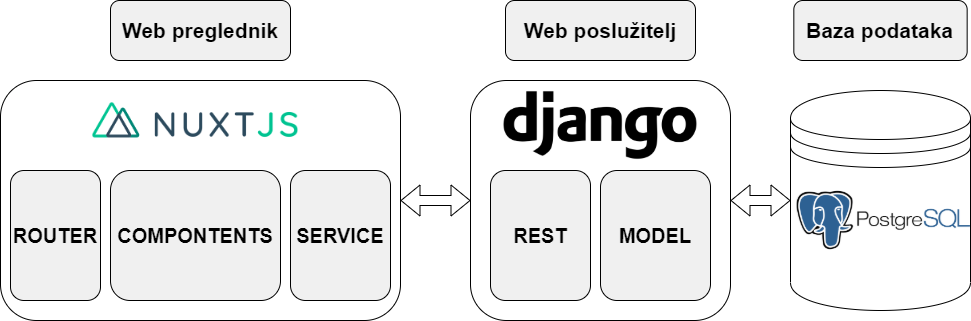
\includegraphics[scale=0.45]{slike/ARHITEKTURA.PNG}
		\caption{Arhitektura sustava}
		\label{fig:promjene}
	\end{figure}	

	\underline{\textit{Web preglednik}} je program čije je svrha omogućiti pregled web-stranice te njenog multimedijalnog sadržaja. Osim samog pregleda, web preglednik mora moći prevesti kod stoga je on ujedinio i kompajler. U našem slučaju web preglednik će prevoditi kod radnog okvira (\emph{engl. framework}) Nuxt.js koje je proširenje Vue.js frameworka.

	\underline{\textit{Web poslužitelj}} je sustav koji treba omogućiti odvijanje komunikacije web preglednika i baze podataka. Njegova zadaća je obrađivati zahtjeve koje zahtjeva web preglednik, po potrebi komunicirati s bazom podataka te vratiti rezultat obrade. Rezultat obrade biti se će SSR (engl. Server Side Rendered) - statički generirana stranica. Komunikacija s poslužiteljem odvija se putem protokola HTTP (\emph{engl. Hyper Text Transfer Protocol}). U našem slučaju za izradu web poslužitelja koristimo Python framework Django koji je besplatan i \emph{open source}.

	\underline{\textit{Baza podataka}} je sustav za trajnu pohranu podataka. U našem slučaju koristimo relacijsku bazu podataka PostgreSQL.

	Zadana arhitektura temelji se na prikazu statički generirane stranice dobivene s web poslužitelja (Django servera). Prema zahtjevu web klijenta Nuxt.js generira zahtjev na API web poslužitelja te dobiva odgovor u obliku generirane statičke stranice. Web poslužitelj prema potrebi šalje zahtjev za dohvat podataka iz baze podataka kako bi mogao stranicu popuniti s relevantnim podacima i multimedijom.

	Django nije tradicionalni MVC (Model-View-Controller) framework, ali se ponaša vrlo slično MVC koncept modelu. MVC koncept model sastoji se od sljedećih komponenata: 
	\begin{packed_item}
		\item{\underline{\textit{Model}} - Dinamičke strukture podataka koje se popunjavaju iz baze podatka za svrhu prikaza ili se popunjavaju iz korisničkog sučelja u svrhu pohrane.}
		\item{\underline{\textit{View}} - Korisničko sučelje preko kojega korisnik podatke prenosi u Model.}
		\item{\underline{\textit{Controller}} - Sučelje između Modela i View-a. Manipulira podacima kako bi ih Model mogao obraditi ili manipulira podatke da ih View može prikazati.}
	\end{packed_item}

	Django razvojni tim preferira koristi koncept MTV (\emph{Model-Template-View}) modela. Razlika između MVC modela i MTV modela je što se komponenta View naziva Template, a komponenta Controller se naziva View.

	\pagebreak
				
	\section{Baza podataka}
			
			\textbf{\textit{dio 1. revizije}}\\
			
		\textit{Potrebno je opisati koju vrstu i implementaciju baze podataka ste odabrali, glavne komponente od kojih se sastoji i slično.}
				
		\noindent Za potrebe našeg sustava koristit ćemo relacijsku bazu podataka PostgreSQL.
		Baza se sastoji od relacija (tablica) i njihovih atributa. Bazu podataka koristimo za pohranu informacija o korisnicima, njihovim rezervacijama i podacima o praonici.
		Baza podataka ove aplikacije sastoji se od sljedećih entiteta:
		\begin{packed_item}
			\item 	Machine
			\item 	Appointment
			\item 	User
			\item 	Post
			\item 	Recension
			\item 	Washday
		\end{packed_item}	
	
		\noindent Osim naših tablica, Django sam stvara nove tablice poput permissiona, sessiona i logova.
		
			\subsection{Opis tablica}
			

				\textit{Svaku tablicu je potrebno opisati po zadanom predlošku. Lijevo se nalazi točno ime varijable u bazi podataka, u sredini se nalazi tip podataka, a desno se nalazi opis varijable. Svjetlozelenom bojom označite primarni ključ. Svjetlo plavom označite strani ključ}
				
				\begin{longtabu} to \textwidth {|X[6, l]|X[6, l]|X[20, l]|}
					
					\hline \multicolumn{3}{|c|}{\textbf{korisnik - ime tablice}}	 \\[3pt] \hline
					\endfirsthead
					
					\hline \multicolumn{3}{|c|}{\textbf{korisnik - ime tablice}}	 \\[3pt] \hline
					\endhead
					
					\hline 
					\endlastfoot
					
					\cellcolor{LightGreen}IDKorisnik & INT	&  	Lorem ipsum dolor sit amet, consectetur adipiscing elit, sed do eiusmod tempor incididunt ut labore et dolore magna aliqua. Ut enim ad minim veniam 	\\ \hline
					korisnickoIme	& VARCHAR &   	\\ \hline 
					email & VARCHAR &   \\ \hline 
					ime & VARCHAR	&  		\\ \hline 
					\cellcolor{LightBlue} primjer	& VARCHAR &   	\\ \hline 
					
					
				\end{longtabu}
			
			\noindent\textbf{Machine}  Ovaj entitet sadrži sve važne informacije vezane za uređaj u praonici. Sadrži atribute: id uređaja i type. Ovaj entitet u vezi je \textit{Many-to-One} s entitetom Appointment preko id-a uređaja.
			
			\begin{longtabu} to \textwidth {|X[8, l]|X[6, l]|X[20, l]|}
				
				\hline \multicolumn{3}{|c|}{\textbf{Machine}}	 \\[3pt] \hline
				\endfirsthead
				
				\hline \multicolumn{3}{|c|}{\textbf{Machine}}	 \\[3pt] \hline
				\endhead
				
				\hline 
				\endlastfoot
				
				\textbf{id} & INT	&  jedinstveni brojčani identifikator	\\ \hline
				type & BOOLEAN &  vrsta uređaja (perilica ili sušilica)\\ \hline 
				
				
			\end{longtabu}
		
			\noindent\textbf{Appointment}  Ovaj entitet sadrži sve važne informacije vezane za rezervirani termin u praonici. Sadrži atribute: id termina, time, machine\_id, price, opcionalni note, paid, basket\_taken, user\_id i employee\_id. Ovaj entitet u vezi je \textit{One-to-Many} s entitetom Machine preko id-a uređaja, vezi \textit{Many-to-One} s entitetom User preko id-a korisnika i id-a zaposlenika.
		
			\begin{longtabu} to \textwidth {|X[8, l]|X[6, l]|X[20, l]|}
				
				\hline \multicolumn{3}{|c|}{\textbf{Appointment}}	 \\[3pt] \hline
				\endfirsthead
				
				\hline \multicolumn{3}{|c|}{\textbf{Appointment}}	 \\[3pt] \hline
				\endhead
				
				\hline 
				\endlastfoot
				\textbf{id} & INT	&  jedinstveni brojčani identifikator	\\ \hline
				time & TIMESTAMP	&  	datum rezerviranog termina u praonici i vrijeme početka 	\\ \hline
				machine\_id (FK)	& INT &  jedinstveni identifikator uređaja kojeg rezerviramo u terminu (machine.id) 	\\ \hline 
				price & FLOAT &  cijena usluge koju korisnik plaća (pranje ili sušenje) \\ \hline 
				note & VARCHAR	& opcionalna bilješka zaposleniku \\ \hline 
				paid & BOOLEAN	& korisnik bira hoće li platiti termin online ili uživo	\\ \hline 
				basket\_taken & BOOLEAN	& korisnik može posuditi jednu košaru iz praonice 	\\ \hline 
				user\_id (FK)	& INT &  jedinstveni identifikator korisnika koji je rezervirao termin (user.id) 	\\ \hline 
				employee\_id (FK)	& INT &  jedinstveni identifikator zaposlenika koji radi za vrijeme rezerviranog termina (user.id)	\\ \hline
				
			\end{longtabu}
		
			\noindent\textbf{User}  Ovaj entitet sadrži sve važne informacije vezane za različite korisnike u praonici. Sadrži atribute: id korisnika, username, password, first\_name, last\_name, jedinstveni JMBAG, jedinstveni email, is\_active, is\_staff, card\_number, negative\_points, date\_joined, last\_login, is\_superuser. Ovaj entitet u vezi je \textit{One-to-Many}  \textit{One-to-Many} s entitetom Appointment preko id-a korisnika, u vezi \textit{One-to-Many} s entitetom Post preko id-a korisnika i u vezi \textit{One-to-Many} s entitetom Recension preko id-a korisnika.
		
			\begin{longtabu} to \textwidth {|X[8, l]|X[6, l]|X[20, l]|}
				
				\hline \multicolumn{3}{|c|}{\textbf{User}}	 \\[3pt] \hline
				\endfirsthead
				
				\hline \multicolumn{3}{|c|}{\textbf{User}}	 \\[3pt] \hline
				\endhead
				
				\hline 
				\endlastfoot
				
				\textbf{id} & INT	&  jedinstveni brojčani identifikator korisnika	\\ \hline
				username	& VARCHAR &   korisničko ime	\\ \hline
				password	& VARCHAR &   lozinka korisničkog računa	\\ \hline
				first\_name	& VARCHAR &   ime korisnika	\\ \hline 
				last\_name	& VARCHAR &   prezime korisnika	\\ \hline
				JMBAG	& VARCHAR &   JMBAG korisnika	\\ \hline
				email	& VARCHAR &   jedinstveni email korisnika	\\ \hline
				is\_active & BOOLEAN &  svi korisnici čije registracije su potvrđene od zaposlenika i koji nisu blokirani\\ \hline 
				is\_staff & BOOLEAN &  oznaka je li korisnik i zaposlenik\\ \hline 
				is\_superuser	& BOOLEAN &   pokazuje je li korisnik ujedno i administrator	\\ \hline
				card\_number	& VARCHAR &   broj kreditne kartice korisnika	\\ \hline
				negative\_points	& INT &   broj negativnih bodova korisnika	\\ \hline
				date\_joined	& DATE &   datum registracije korisnika	\\ \hline
				last\_login	& TIMESTAMP &  vrijeme zadnje prijave u sustav	\\ \hline
			
				
				
			\end{longtabu}
		
			\noindent\textbf{Post}  Ovaj entitet sadrži sve važne informacije vezane za objavu. Sadrži atribute: id objave, photo, text, date, type i employee\_id. 
			Ovaj entitet u vezi je \textit{Many-to-One} s entitetom User preko id-a zaposlenika.
		
			\begin{longtabu} to \textwidth {|X[8, l]|X[6, l]|X[20, l]|}
				
				\hline \multicolumn{3}{|c|}{\textbf{Post}}	 \\[3pt] \hline
				\endfirsthead
				
				\hline \multicolumn{3}{|c|}{\textbf{Post}}	 \\[3pt] \hline
				\endhead
				
				\hline 
				\endlastfoot
				
				\textbf{id} & INT	&  jedinstveni brojčani identifikator objave	\\ \hline
				photo	& BYTEA &   opcionalna slika priložena uz objavu	\\ \hline 
				text	& VARCHAR &   tekst objave	\\ \hline
				date	& DATE &  datum objavljivanja objave	\\ \hline
				type	& BOOLEAN &   ako je vrijednost zastavice 1, objava se prikazuje na "LostAndFound" stranici 	\\ \hline
				employee\_id (FK)	& INT &  id zaposlenika koji radi za vrijeme rezerviranog termina (user.id) 	\\ \hline		
						
				
				
			\end{longtabu}
		
			\noindent\textbf{Recension}  Ovaj entitet sadrži sve važne informacije vezane za recenzije. Sadrži atribute: id recenzije, user\_id, employee\_id, text i grade. Ovaj entitet u vezi je \textit{Many-to-One} s entitetom User preko id-a zaposlenika i id-a korisnika.
		
			\begin{longtabu} to \textwidth {|X[8, l]|X[6, l]|X[20, l]|}
				
				\hline \multicolumn{3}{|c|}{\textbf{Recension}}	 \\[3pt] \hline
				\endfirsthead
				
				\hline \multicolumn{3}{|c|}{\textbf{Recension}}	 \\[3pt] \hline
				\endhead
				
				\hline 
				\endlastfoot
				
				\textbf{id} & INT	&  jedinstveni brojčani identifikator recenzije	\\ \hline
				user\_id (FK)	& INT &  id korisnika koji je ostavio recenziju (user.id) 	\\ \hline
				employee\_id (FK)	& INT &  id recenziranog zaposlenika (user.id)	\\ \hline
				text	& VARCHAR &   tekst recenzije	\\ \hline
				grade	& INT & ocjena zaposlenika od 1 do 5	\\ \hline
				
			\end{longtabu}
			
			\noindent\textbf{Washday}  Ovaj entitet sadrži sve važne informacije vezane za radni dan praonice. Sadrži atribute: id radnog dana, date, open\_time, close\_time, pause\_start, pause\_end i wash\_price. Ovaj entitet nije u vezi ni s jednim drugim entitetom.
			
			\begin{longtabu} to \textwidth {|X[8, l]|X[6, l]|X[20, l]|}
				
				\hline \multicolumn{3}{|c|}{\textbf{Washday}}	 \\[3pt] \hline
				\endfirsthead
				
				\hline \multicolumn{3}{|c|}{\textbf{Washday}}	 \\[3pt] \hline
				\endhead
				
				\hline 
				\endlastfoot
				
				\textbf{id} & INT	&  jedinstveni brojčani  identifikator radnog dana praonice	\\ \hline
				date & DATE	&  trenutni datum	\\ \hline
				open\_time	& TIME &   početak radnog vremena	\\ \hline
				close\_time	& TIME & kraj radnog vremena	\\ \hline
				pause\_start	& TIME & početak pauze	\\ \hline
				pause\_end	& TIME & kraj pauze	\\ \hline
				wash\_price	& FLOAT & cijena jednog pranja	\\ \hline
				drying\_price	& FLOAT & cijena jednog sušenja	\\ \hline
				
				
			\end{longtabu}
			
			
			\subsection{Dijagram baze podataka}
				\textit{ U ovom potpoglavlju potrebno je umetnuti dijagram baze podataka. Primarni i strani ključevi moraju biti označeni, a tablice povezane. Bazu podataka je potrebno normalizirati. Podsjetite se kolegija "Baze podataka".}
				
				\begin{figure}[H]
					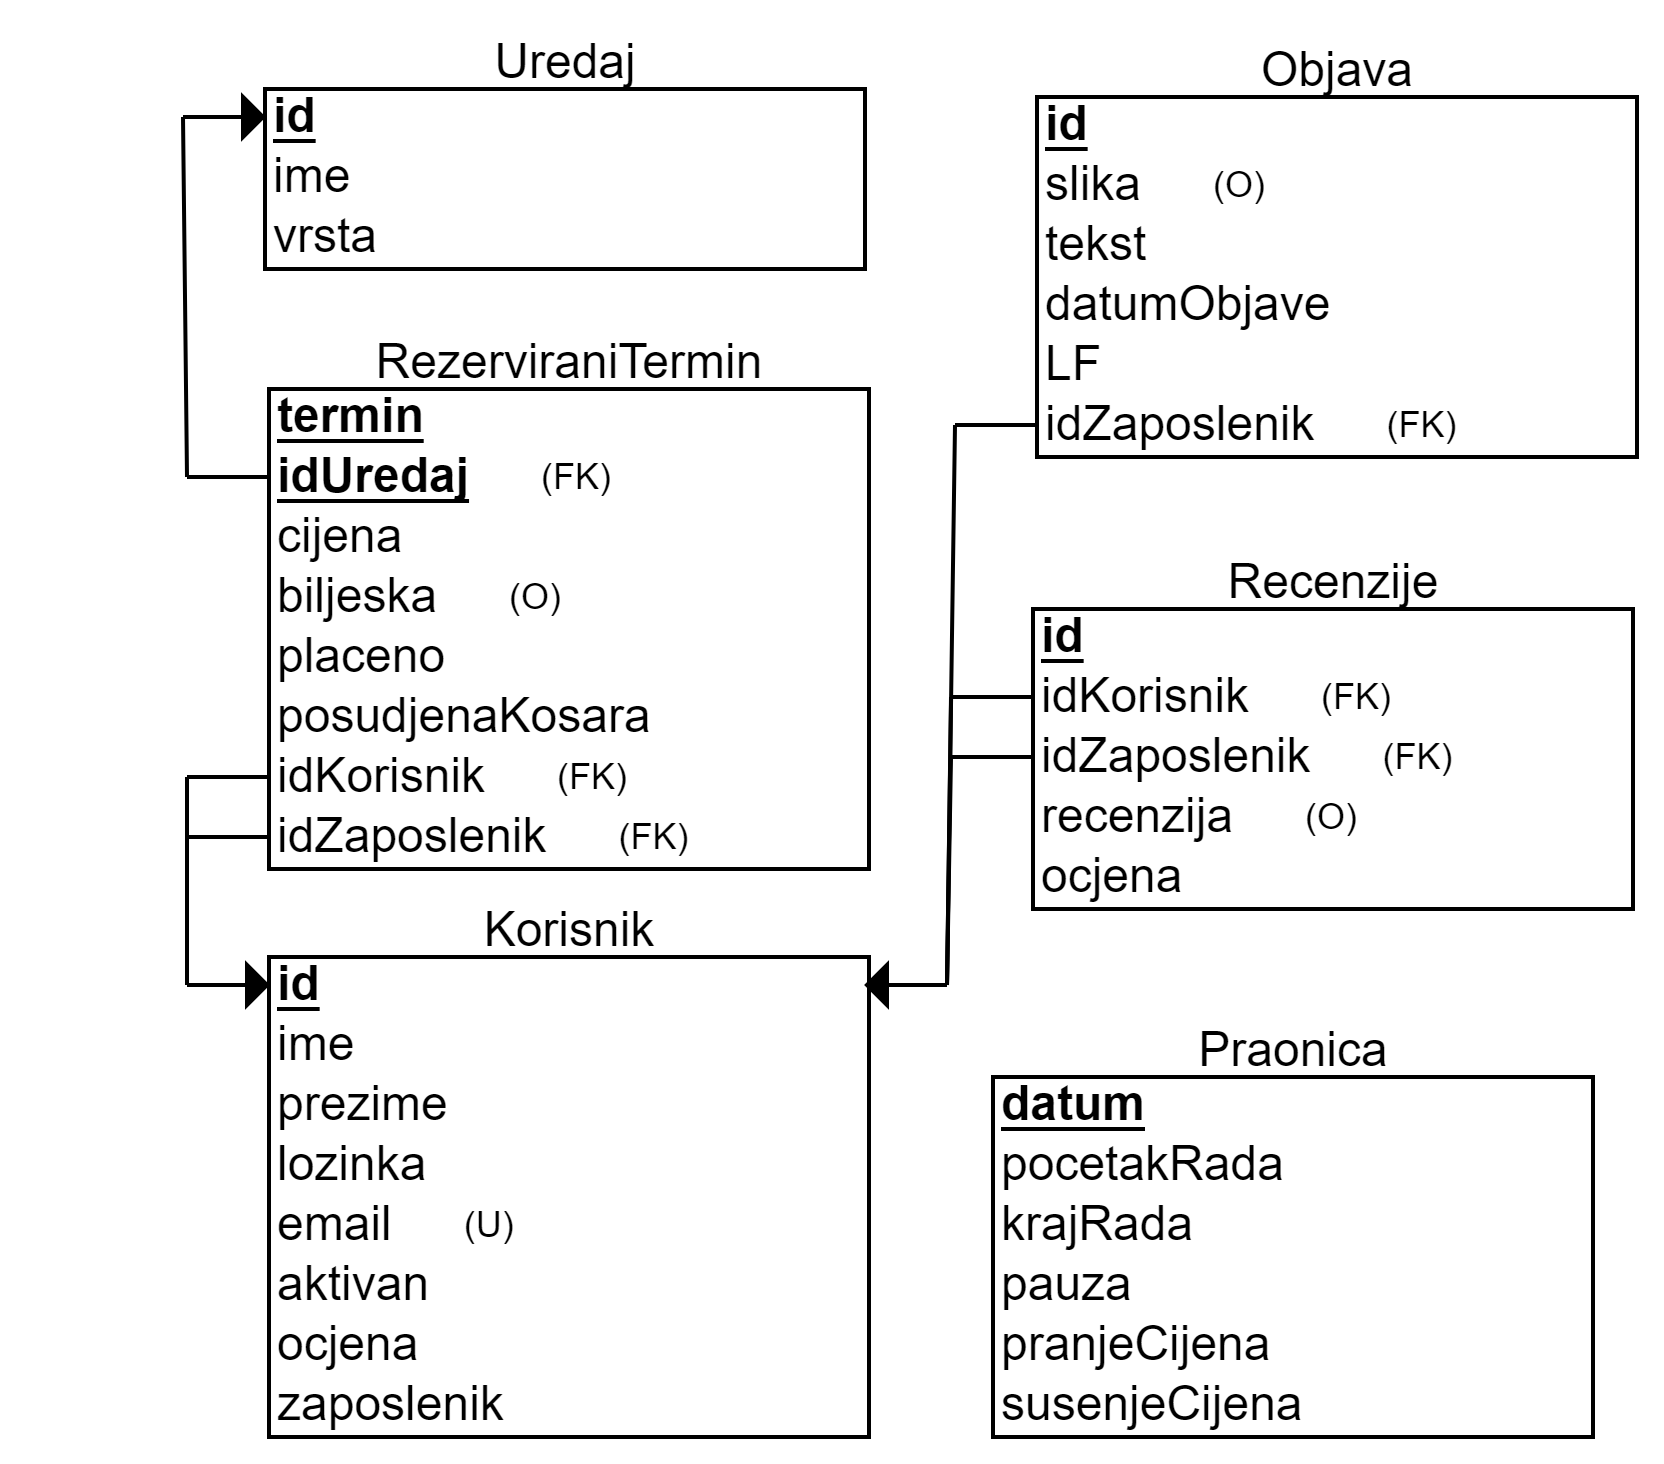
\includegraphics[scale=0.2]{slike/BAZA.PNG} %veličina slike u odnosu na originalnu datoteku i pozicija slike
					\centering
					\caption{Relacijska shema baze podataka}
					\label{fig:promjene}
				\end{figure}
			\eject
			
			
			\begin{figure}[H]
				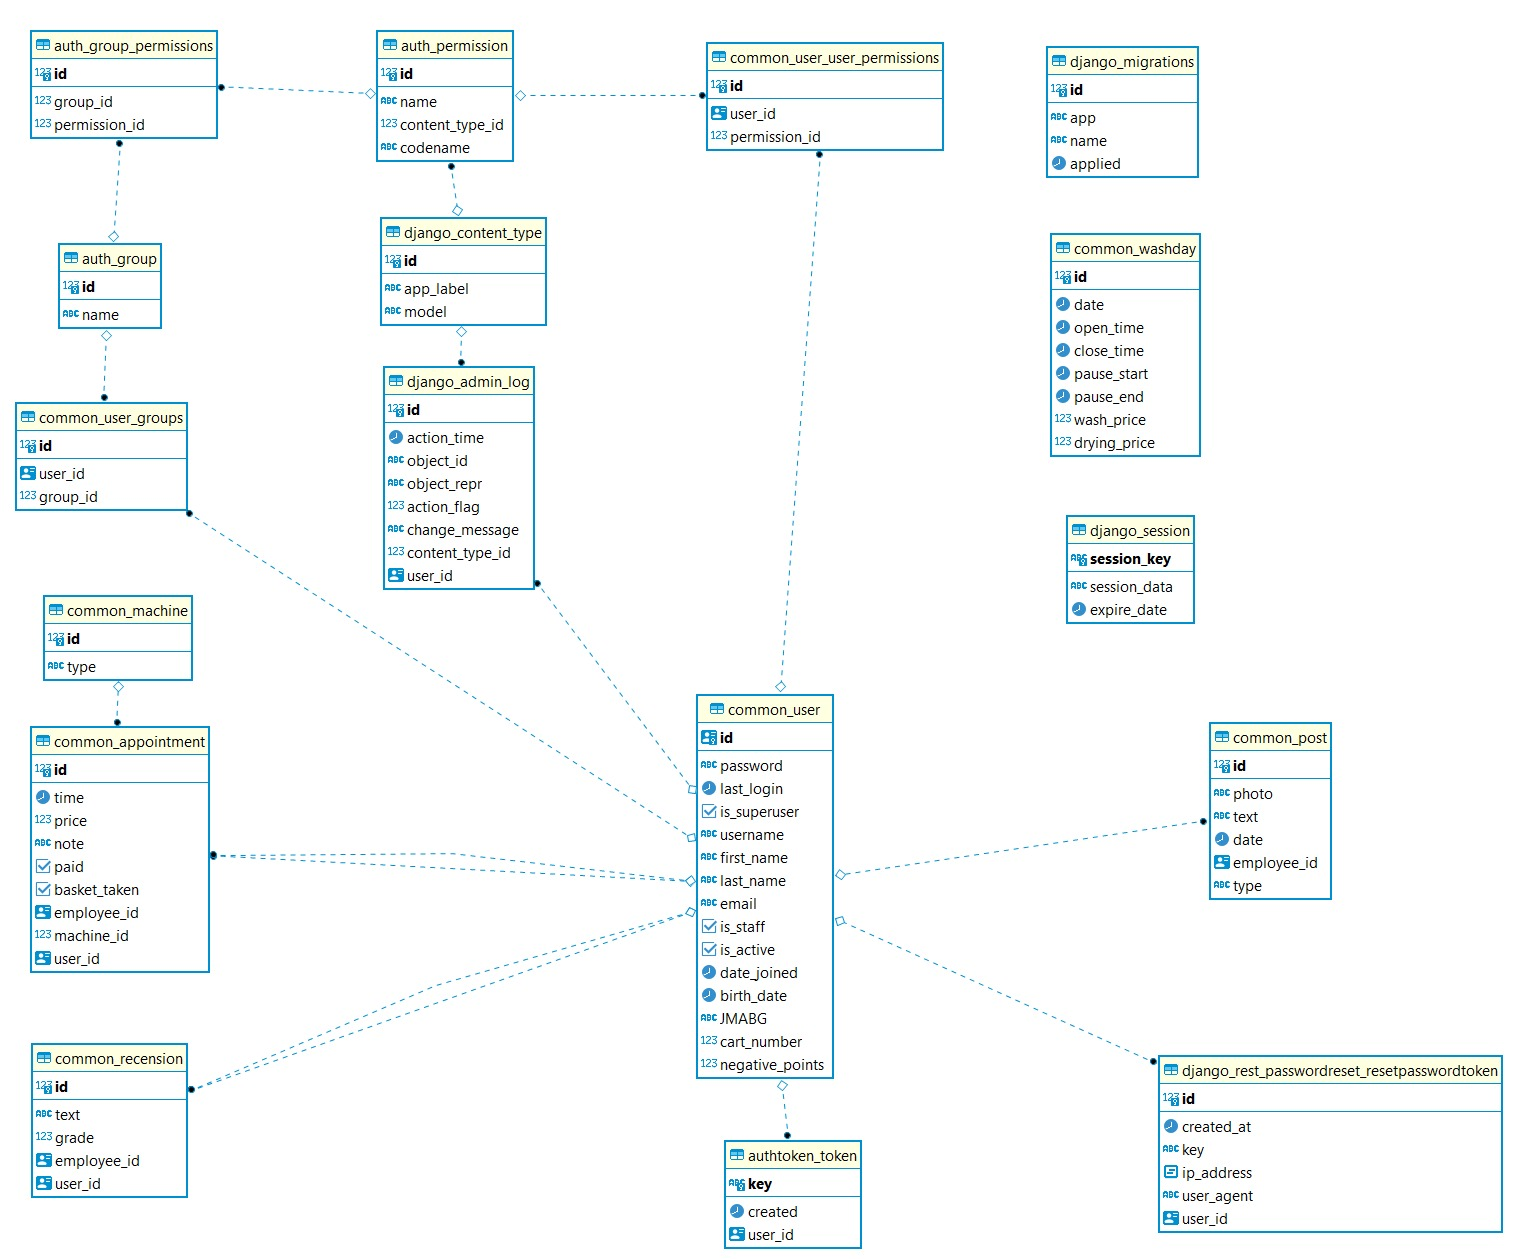
\includegraphics[scale=0.3]{slike/djangoBaza.jpeg} %veličina slike u odnosu na originalnu datoteku i pozicija slike
				\centering
				\caption{Relacijska shema Django baze podataka}
				\label{fig:promjene}
			\end{figure}
			\eject
			
			
		\section{Dijagram razreda}
		
			\textit{Potrebno je priložiti dijagram razreda s pripadajućim opisom. Zbog preglednosti je moguće dijagram razlomiti na više njih, ali moraju biti grupirani prema sličnim razinama apstrakcije i srodnim funkcionalnostima.}\\
			
			\textbf{\textit{dio 1. revizije}}\\
			
			\textit{Prilikom prve predaje projekta, potrebno je priložiti potpuno razrađen dijagram razreda vezan uz \textbf{generičku funkcionalnost} sustava. Ostale funkcionalnosti trebaju biti idejno razrađene u dijagramu sa sljedećim komponentama: nazivi razreda, nazivi metoda i vrste pristupa metodama (npr. javni, zaštićeni), nazivi atributa razreda, veze i odnosi između razreda.}\\
			
			\textbf{\textit{dio 2. revizije}}\\			
			
			\textit{Prilikom druge predaje projekta dijagram razreda i opisi moraju odgovarati stvarnom stanju implementacije} \\
			
			Zbog toga što je web poslužitelj napisan u Pythonu, ne možemo reći da u našem web modelu postoje razredi u pravom smislu riječi. Naime, moguće je pisati razred u Pythonu, ali nije moguće koristiti vrste pristupa. Sve metode, razredi i atributi su javne (i tako će biti označene na dijagramima). Moguće je naznačiti da želimo da se komponenta ponaša kao privatna korištenjem donje crtice u njenom imenu. Stoga zaključujemo da razredi u Pythonu postoje i moguće je izraditi dijagram razreda za komponente web aplikacije iako razredi nemaju potpune funkcionalnosti objektno orijentiranog jezika. Django koristi razrede prilikom svoje implementacije. Kao što je već navedeno, Django se temelji na modelu MTV (\emph{Model-Template-View}).\\\
			
			\pagebreak
			\emph{Models} u Djangu su Python razredi koji se automatski prenose u obliku relacija u bazu podataka korištenjem Djangovih karakterističnih \emph {migrate} funkcionalnosti.  Prilikom pisanja Modela potrebno je obratiti pozornost na njihovu povezanost i buduću brojnost u bazi podataka. 	
			\begin{figure}[H]
				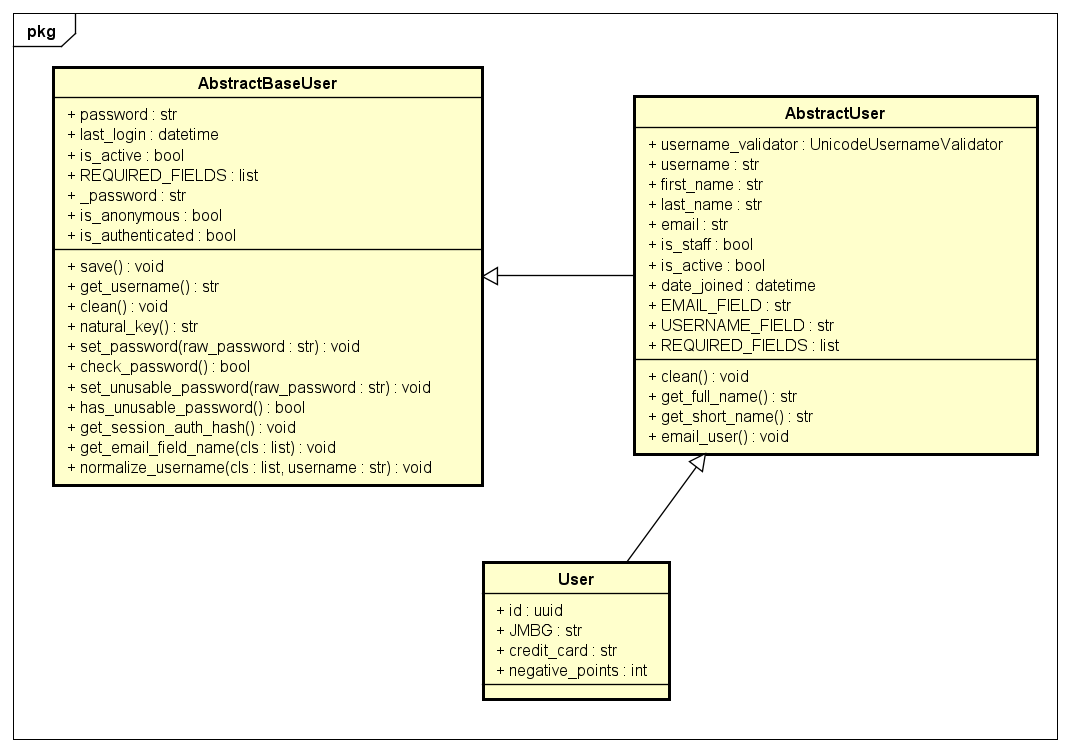
\includegraphics[scale=0.55]{slike/Razredni_dijagrami_Models.PNG} 
				\centering
				\caption{Dijagram razreda - dio Models}
				\label{fig:promjene}
			\end{figure}
		
			\pagebreak
			\emph{Views} sadrže svu funkcionalnost i strukture podataka potrebne da se povežu funkcionalnosti Templatea i Modela. Osim što povezuju ta dva dijela sustava, views mogu sadržavati dodatnu funkcionalnost.
			\begin{figure}[H]
				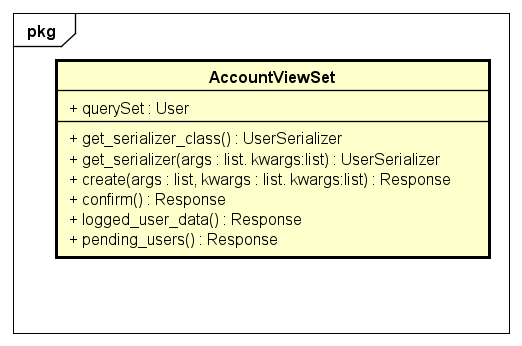
\includegraphics[scale=0.55]{slike/Razredni_dijagrami_Views.PNG}
				\centering
				\caption{Dijagram razreda - dio Views}
				\label{fig:promjene}
			\end{figure}  	
		
		 	\pagebreak			
 			\emph{Templates} sadrže sve strukture podataka potrebne da se podatak prenese s korisničkog sučelja u model. U našem slučaju korisničko sučelje dio je Nuxt.js radnog okvira. Nuxt.js uz pomoć \emph{axios} sustava prenosi podatke na View.
 			\begin{figure}[H]
 				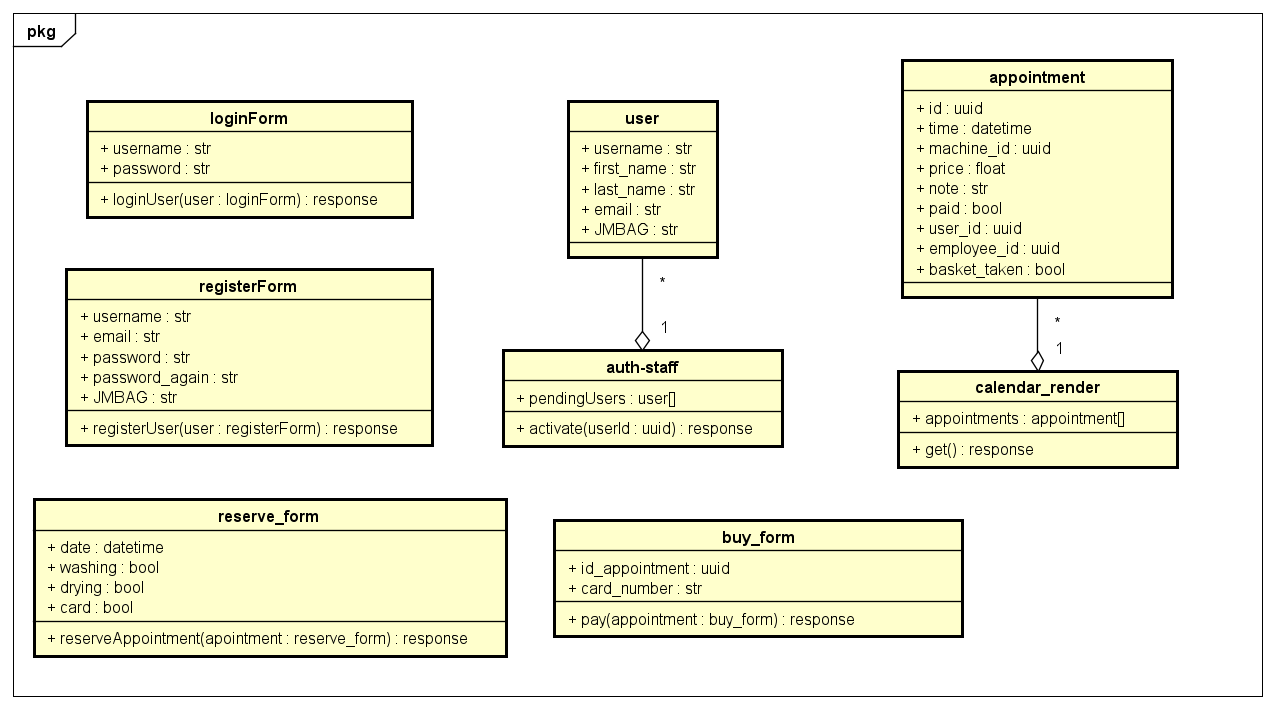
\includegraphics[scale=0.45]{slike/Razredni_dijagrami_Templates.PNG}
 				\centering
 				\caption{Dijagram razreda - dio Templates}
 				\label{fig:promjene}
 			\end{figure} 	
 		
			\pagebreak
 			
 			
		\section{Dijagram stanja}
			
			
			\textbf{\textit{dio 2. revizije}}\\
			
			\textit{Potrebno je priložiti dijagram stanja i opisati ga. Dovoljan je jedan dijagram stanja koji prikazuje \textbf{značajan dio funkcionalnosti} sustava. Na primjer, stanja korisničkog sučelja i tijek korištenja neke ključne funkcionalnosti jesu značajan dio sustava, a registracija i prijava nisu. }
			
			
			\eject 
		
		\section{Dijagram aktivnosti}
			
			\textbf{\textit{dio 2. revizije}}\\
			
			 \textit{Potrebno je priložiti dijagram aktivnosti s pripadajućim opisom. Dijagram aktivnosti treba prikazivati značajan dio sustava.}
			
			\eject
		\section{Dijagram komponenti}
		
			\textbf{\textit{dio 2. revizije}}\\
		
			 \textit{Potrebno je priložiti dijagram komponenti s pripadajućim opisom. Dijagram komponenti treba prikazivati strukturu cijele aplikacije.}
	\chapter{Implementacija i korisničko sučelje}
		
		
		\section{Korištene tehnologije i alati}
			
			
			Komunikacija u timu realizirana je korištenjem aplikacije WhatsApp\footnote{\url{https://www.whatsapp.com/}}, a organizacija i podjela zadataka korištenjem aplikacije Trello\footnote{\url{https://trello.com/}}. 
			Za izradu UML dijagrama korišten je alat Astah UML\footnote{\url{https://astah.net/products/astah-uml/}}, a kao sustav za upravljanje
			izvornim kodom Git\footnote{\url{https://git-scm.com/}}. Udaljeni repozitorij projekta dostupan je na web platformi
			GitLab\footnote{\url{https://gitlab.com/}}.
			
			Kao razvojno okruženje korišten je Microsoft Visual Studio Code\footnote{\url{https://code.visualstudio.com/}} - 
			besplatni uređivač teksta tvrtke Microsoft. Sadrži podršku za debugging, izvođenje zadataka te sustav za upravljanje izvornim kodom. Koristi se za razvoj računalnih
			programa za operacijski sustav Windows, kao i za web-stranice, web-aplikacije,
			te ostale web-usluge. Jedan je od najpopularnijih razvojnih alata. Bazira se na radnom sučelju Electron, koje se koristi za razvoj Node.js Web aplikacija.
			
			
			Aplikacija je napisana koristeći radni okvir Django\footnote{\url{https://www.djangoproject.com/}} i jezik Python\footnote{\url{https://www.python.org/}} za
			izradu backenda te Nuxt.js\footnote{\url{https://nuxtjs.org/}} i jezik JavaScript\footnote{\url{https://www.javascript.com/}} za izradu frontenda. Nuxt.js je radni okvir koji se bazira na Vue.js\footnote{\url{https://vuejs.org/}}, Node.js\footnote{\url{https://nodejs.org/en/}}, Webpack\footnote{\url{https://webpack.js.org/}} i Babel.js\footnote{\url{https://babeljs.io/}}. Podržava generiranje statičkih web stranica i bazira se na modularnoj arhitekturi. Postoji preko 50 modula koji razvoj čine bržim i jednostavnijim. Django radni okvir omogućava brz razvoj sigurnih i održivih web stranica. Prati MTV (model-template-view) arhitekturni obrazac. Neke od poznatih stranica koje koriste Django su Instagram, Mozilla, The Washington Times, Bitbucket itd.
			
			Za lokalno upravljanje i slanje upita na bazu podataka koristili smo alat pgAdmin\footnote{\url{https://www.pgadmin.org/}}. Baza podataka se trenutno nalazi na poslužitelju Heroku\footnote{\url{https://www.heroku.com/}}.
			
			
			
			
			\eject 
		
	
		\section{Ispitivanje programskog rješenja}
			
			\textbf{\textit{dio 2. revizije}}\\
			
			 \textit{U ovom poglavlju je potrebno opisati provedbu ispitivanja implementiranih funkcionalnosti na razini komponenti i na razini cijelog sustava s prikazom odabranih ispitnih slučajeva. Studenti trebaju ispitati temeljnu funkcionalnost i rubne uvjete.}
	
			
			\subsection{Ispitivanje komponenti}
			U ovom ćemo poglavlju predstaviti 9 ispitnih slučajeva (unit testova). Svi se ispitni primjeri mogu pronaći u datoteci janezi/izvorniKod/backend/common/tests.py koja je sastavljena od 4 klase koje ukupno sadrže 9 testova te sadrži 137 linija programskog koda.
			
			\vspace{5mm} %5mm vertical space
			
			Ispitni slučajevi 1 i 2 odnose se na prijavu korisnika. Oba se ispitna slučaja nalaze u klasi AccountTests. U prvom se slučaju korisnik ne može prijaviti jer mu korisnički račun nije potvrđen, dok se u drugom slučaju, odmah nakon potvrde računa, korisnik može uspješno prijaviti. U prvom je slučaju očekivan odgovor 400 (pogreška), dok je u drugom slučaju očekivan odgovor 200. Oba ispitna primjera daju očekivani rezultat.
			
			\begin{figure}[H]
				\centering
				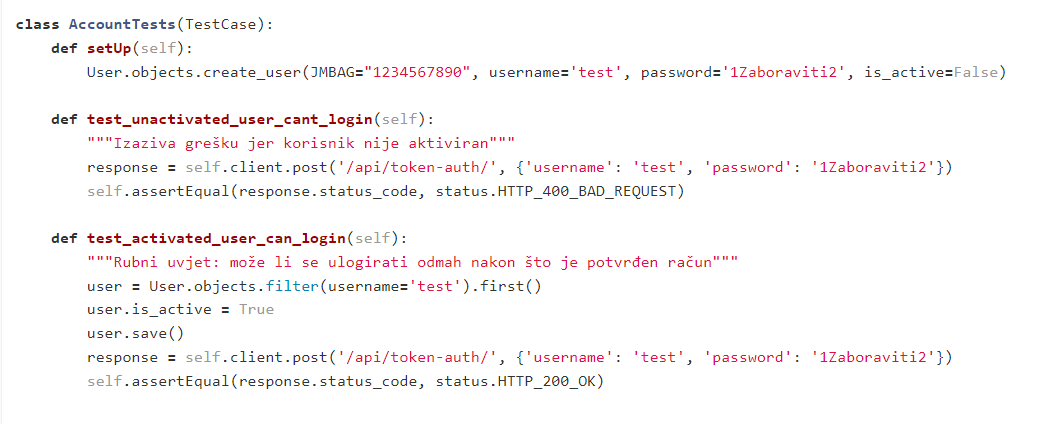
\includegraphics[scale=0.65]{slike/AccountTests.PNG}
				\caption{Ispitni slučajevi vezani za prijavu korisnika}
				\label{fig:promjene}
			\end{figure}
		
			Ispitni slučajevi 3 i 4 vezani su za administratora te provjeravaju ispravnost funkcionalnosti blokiranja korisnika. Oba se ispitna slučaja nalaze u klasi AdminTests. Prvi slučaj izaziva pogrešku (kod 401 UNAUTHORIZED) jer korisnik koji nije administrator pokušava blokirati račun drugog korisnika. U drugom slučaju, korisnik koji je administrator blokira korisnika i provjerava se točnost akcije. Oba ispitna primjera daju očekivani rezultat.
			
			\begin{figure}[H]
				\centering
				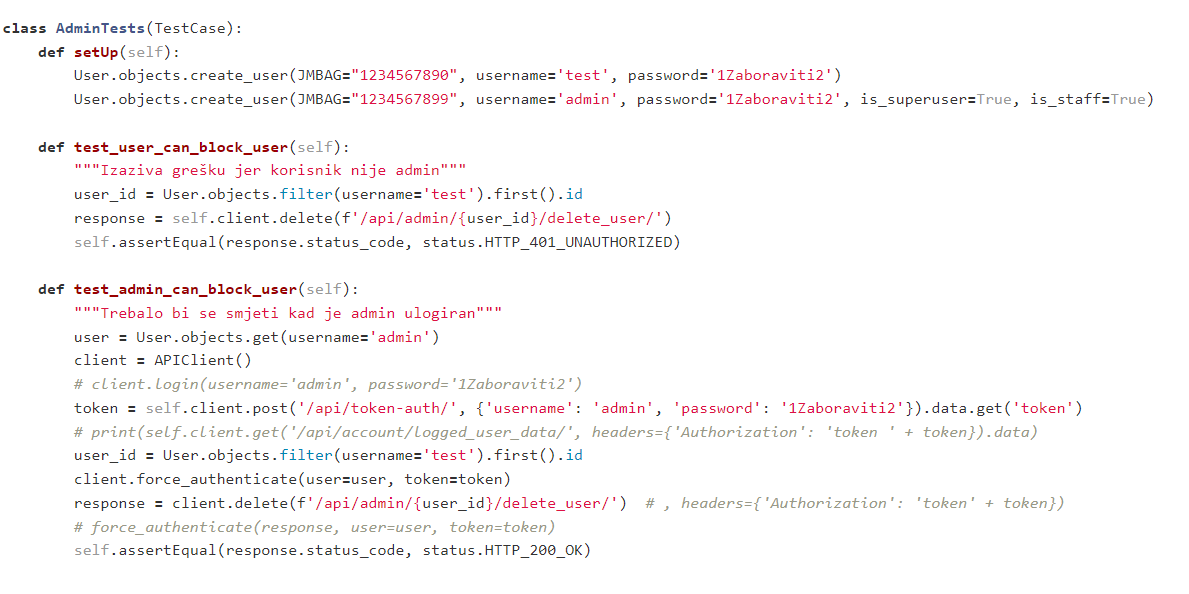
\includegraphics[scale=0.65]{slike/AdminTests.PNG}
				\caption{Ispitni slučajevi vezani za prijavu korisnika}
				\label{fig:promjene}
			\end{figure}
	
			Ispitni slučajevi 5, 6 i 7 odnose se na funkcionalnost vraćanja košare. Oba se ispitna slučaja nalaze u klasi WorkerTests. Prvi slučaj predstavlja situaciju u kojoj korisnik koji ne radi u praonici pokušava vratiti košaru. Taj bi slučaj trebao vratiti poruku 401 UNAUTHORIZED kako netko ne bi mogao zloupotrebljavati povrat košare. Drugi test provjerava ponašanje aplikacije u slučaju kad radnik pokuša označiti da je netko vratio košaru te osim provjere uspješnosti (kod 200), provjerava se i je li se broj košara tog korisnika smanjio na 0 (linija 75 u kodu). Sva tri ispitna primjera daju rezultat u skladu s očekivanjima.
			
			\begin{figure}[H]
				\centering
				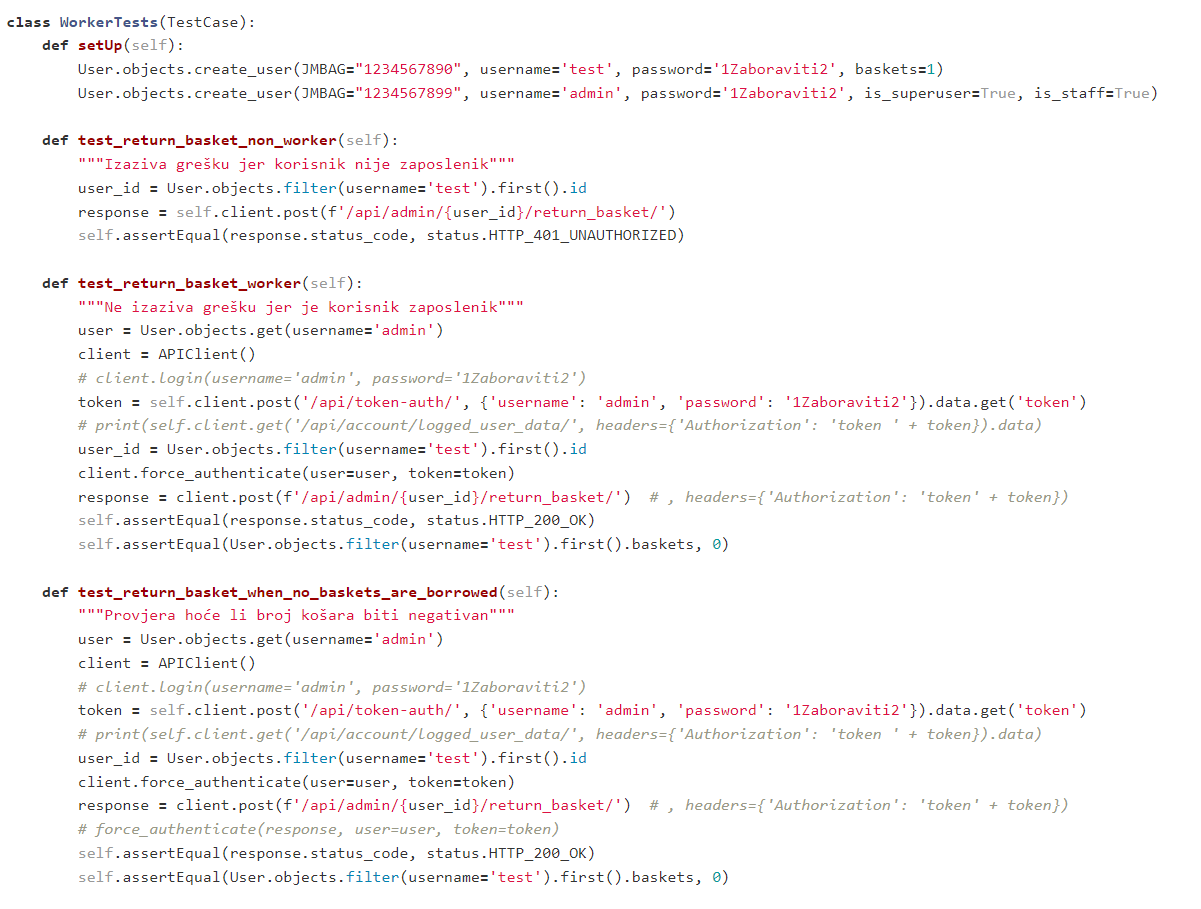
\includegraphics[scale=0.65]{slike/WorkerTests.PNG}
				\caption{Ispitni slučajevi vezani za vraćanje košara}
				\label{fig:promjene}
			\end{figure}
		
			Posljednja klasa ispitnih primjera, nalazi se u klasi AppointmentTests i sadrži ispitne primjere 8 i 9. Osmi ispitni primjer provjerava može li neregistrirani korisnik napraviti rezervaciju te je očekivano ponašanje pogreška s kodom 401. Ispitni primjer br. 9 ispituje rezervaciju termina nakon prijave i provjerava je li radnja bila uspješna (kod 201 CREATED). Oba ispitna primjera daju očekivani rezultat.
			
			\begin{figure}[H]
				\centering
				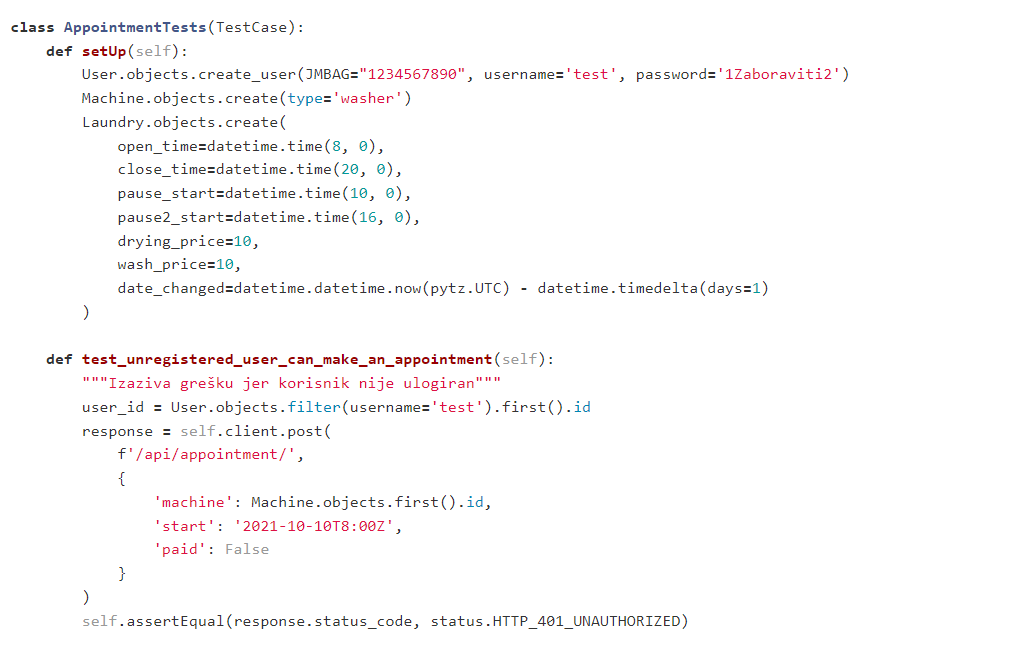
\includegraphics[scale=0.65]{slike/AppointmentTests1.PNG}
				\caption{Ispitni slučajevi vezani za rezervaciju termina, slika 1/2}
				\label{fig:promjene}
			\end{figure}
		
			\begin{figure}[H]
				\centering
				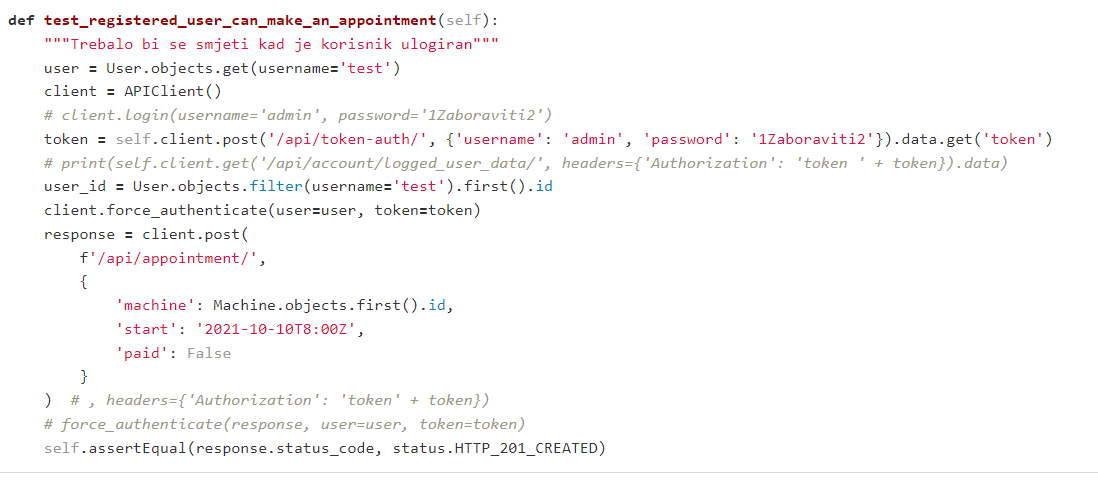
\includegraphics[scale=0.65]{slike/AppointmentTests2.PNG}
				\caption{Ispitni slučajevi vezani za rezervaciju termina, slika 2/2}
				\label{fig:promjene}
			\end{figure}
		
			Svi se spomenuti testovi mogu pokrenuti iz terminala aktivacijom virtualnog okruženja, pozicioniranjem u mapu backend i pozivanjem naredbe ./manage.py test. Kao što je već spomenuto, svi se testovi izvršavaju točno, a slika ~\ref{fig:TestsTerminal} pokretanja naredbe ./manage.py test dana je u prilogu. 
			
			\begin{figure}[H]
				\centering
				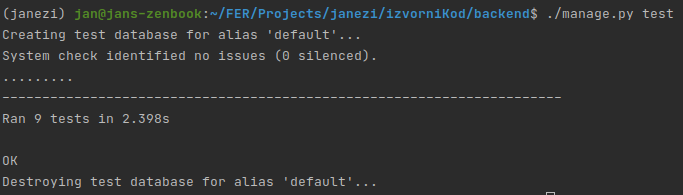
\includegraphics[scale=0.65]{slike/TestsTerminal.PNG}
				\caption{Pokretanje svih ispitnih slučajeva u terminalu}
				\label{fig:TestsTerminal}
			\end{figure}
			
			
			\subsection{Ispitivanje sustava}
			
			 \textit{Potrebno je provesti i opisati ispitivanje sustava koristeći radni okvir Selenium\footnote{\url{https://www.seleniumhq.org/}}. Razraditi \textbf{minimalno 4 ispitna slučaja} u kojima će se ispitati redovni slučajevi, rubni uvjeti te poziv funkcionalnosti koja nije implementirana/izaziva pogrešku kako bi se vidjelo na koji način sustav reagira kada nešto nije u potpunosti ostvareno. Ispitni slučaj se treba sastojati od ulaza (npr. korisničko ime i lozinka), očekivanog izlaza ili rezultata, koraka ispitivanja i dobivenog izlaza ili rezultata.\\ }
			 
			 \textit{Izradu ispitnih slučajeva pomoću radnog okvira Selenium moguće je provesti pomoću jednog od sljedeća dva alata:}
			 \begin{itemize}
			 	\item \textit{dodatak za preglednik \textbf{Selenium IDE} - snimanje korisnikovih akcija radi automatskog ponavljanja ispita	}
			 	\item \textit{\textbf{Selenium WebDriver} - podrška za pisanje ispita u jezicima Java, C\#, PHP koristeći posebno programsko sučelje.}
			 \end{itemize}
		 	\textit{Detalji o korištenju alata Selenium bit će prikazani na posebnom predavanju tijekom semestra.}
			
			\eject 
		
		
		\section{Dijagram razmještaja}
			Na poslužiteljskom računalu se nalaze web poslužitelj i poslužitelj baze podataka. Oni se nalaze unutar Heroku izvršne okoline koja sadrži usluge koje organiziraju i upravljaju izvršavanjem i razmjerom aplikacije. Frontend i backend se pokreću u Dynosima. To su lagana, izolirana okruženja koja pružaju računalnu snagu, memoriju, OS i "Ephemeral" datotečni sustav. Klijenti koriste web preglednik kako bi pristupili web aplikaciji.  Sustav je baziran na arhitekturi ”klijent-poslužitelj”, a komunikacija između računala korisnika (klijent, zaposlenik, administrator) i poslužitelja odvija se preko HTTPS veze.
			
			\begin{figure}[H]
				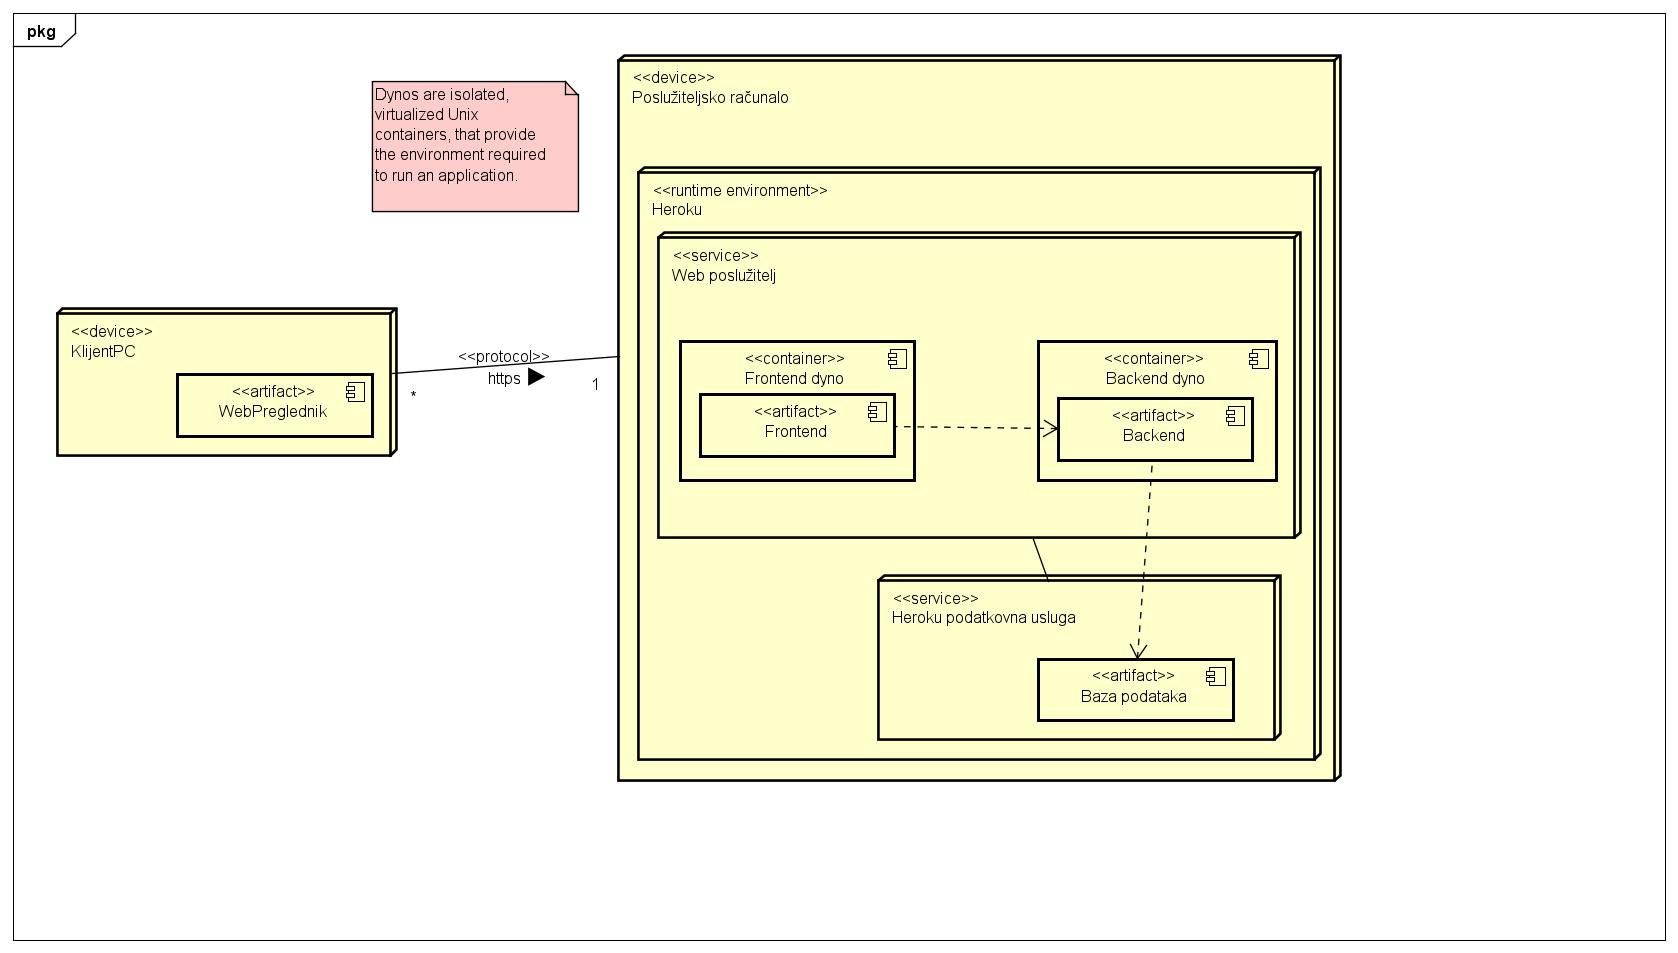
\includegraphics[width=1\linewidth]{slike/dijagram-razmjestaja.jpg}
				\centering
				\caption{Dijagram stanja}
				\label{fig:dijagram_razmjestaja}
			\end{figure}
			\eject 
		
		\section{Upute za puštanje u pogon}
		
			Za puštanje u pogon, koristili smo heroku server (https://www.heroku.com/). Prvi korak za puštanje u pogon bila je podjela aplikacije na poslužiteljsku i korisničku stranu. Svaki se od tih djelova aplikacije treba staviti u zasebnu mapu. Imena mapi moraju odgovarati imenima aplikacija na heroku poslužitelju. Mi smo se odlučili za naziv terminko za korisničku stranu te naziv terminko1 za poslužiteljsku stranu.
			
			\begin{figure}[H]
				\centering
				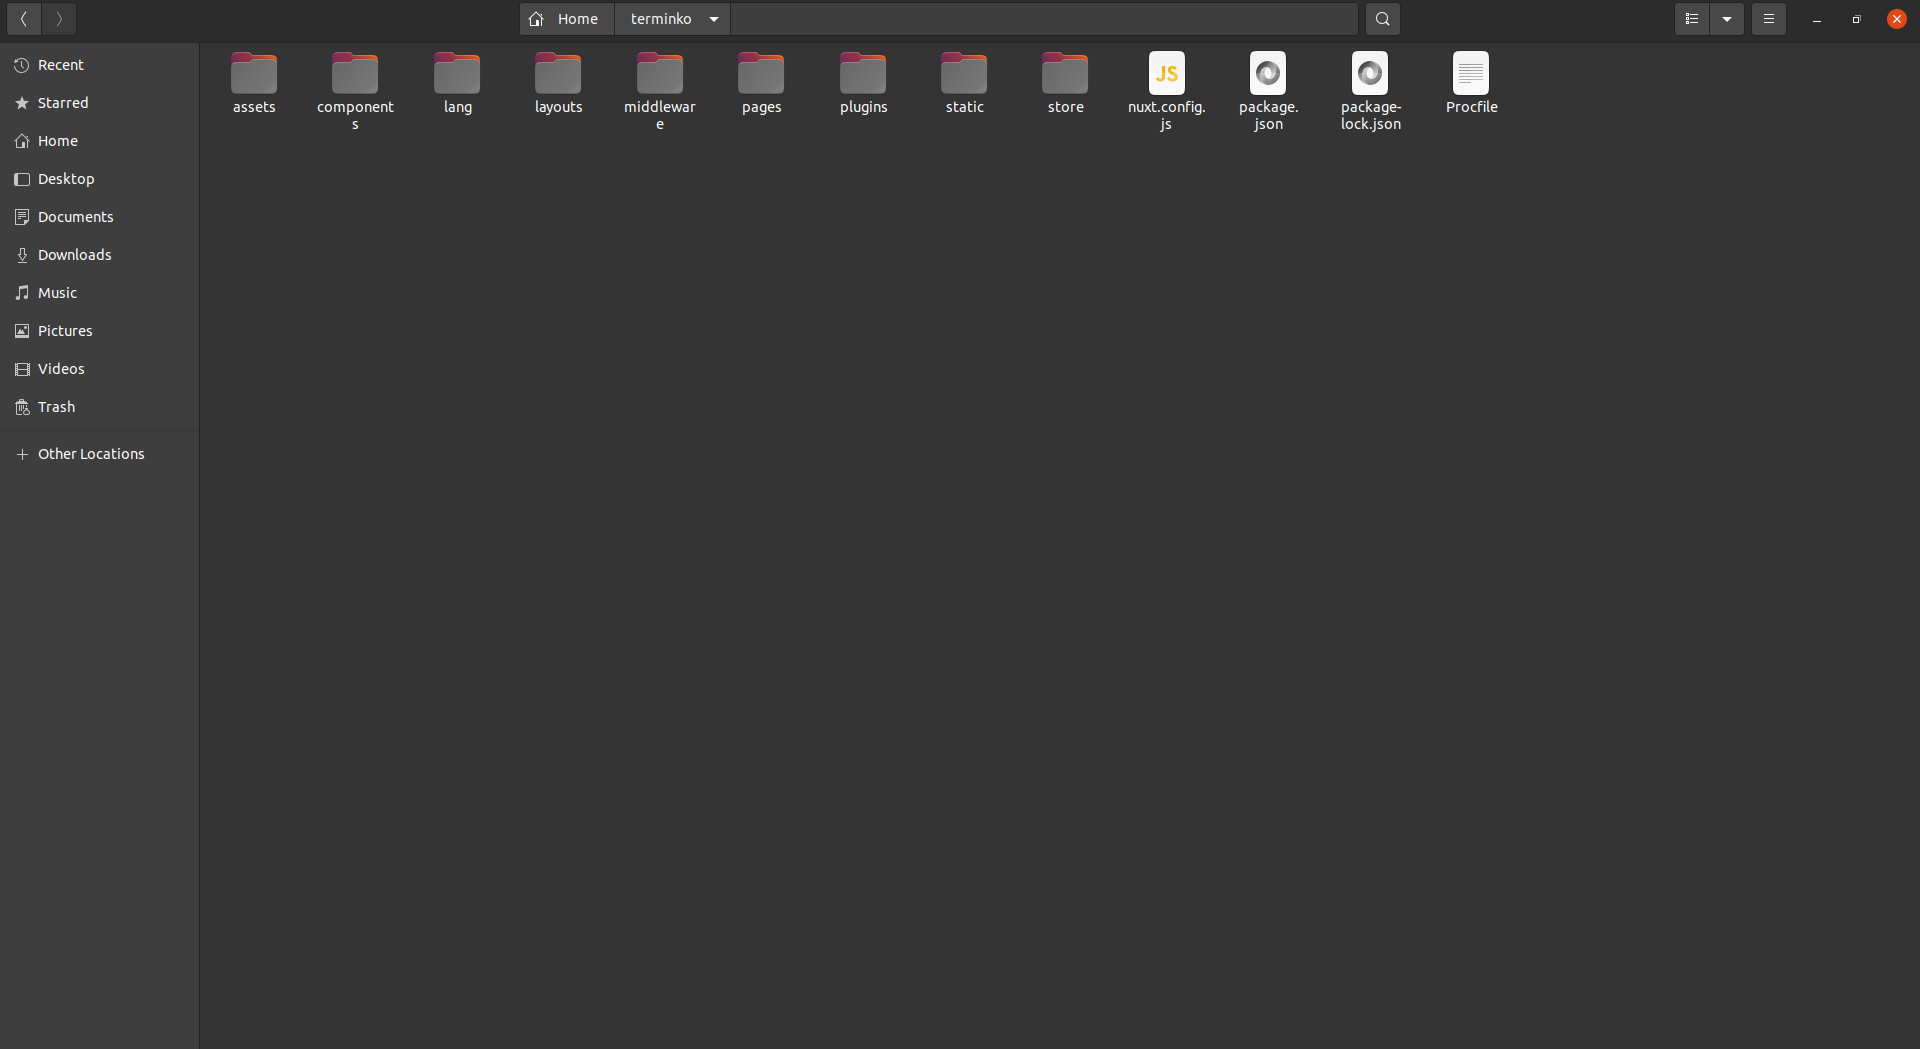
\includegraphics[scale=0.25]{slike/FrontendMapa.PNG}
				\caption{Mapa za frontend: terminko}
				\label{fig:promjene}
			\end{figure}
			
			\begin{figure}[H]
				\centering
				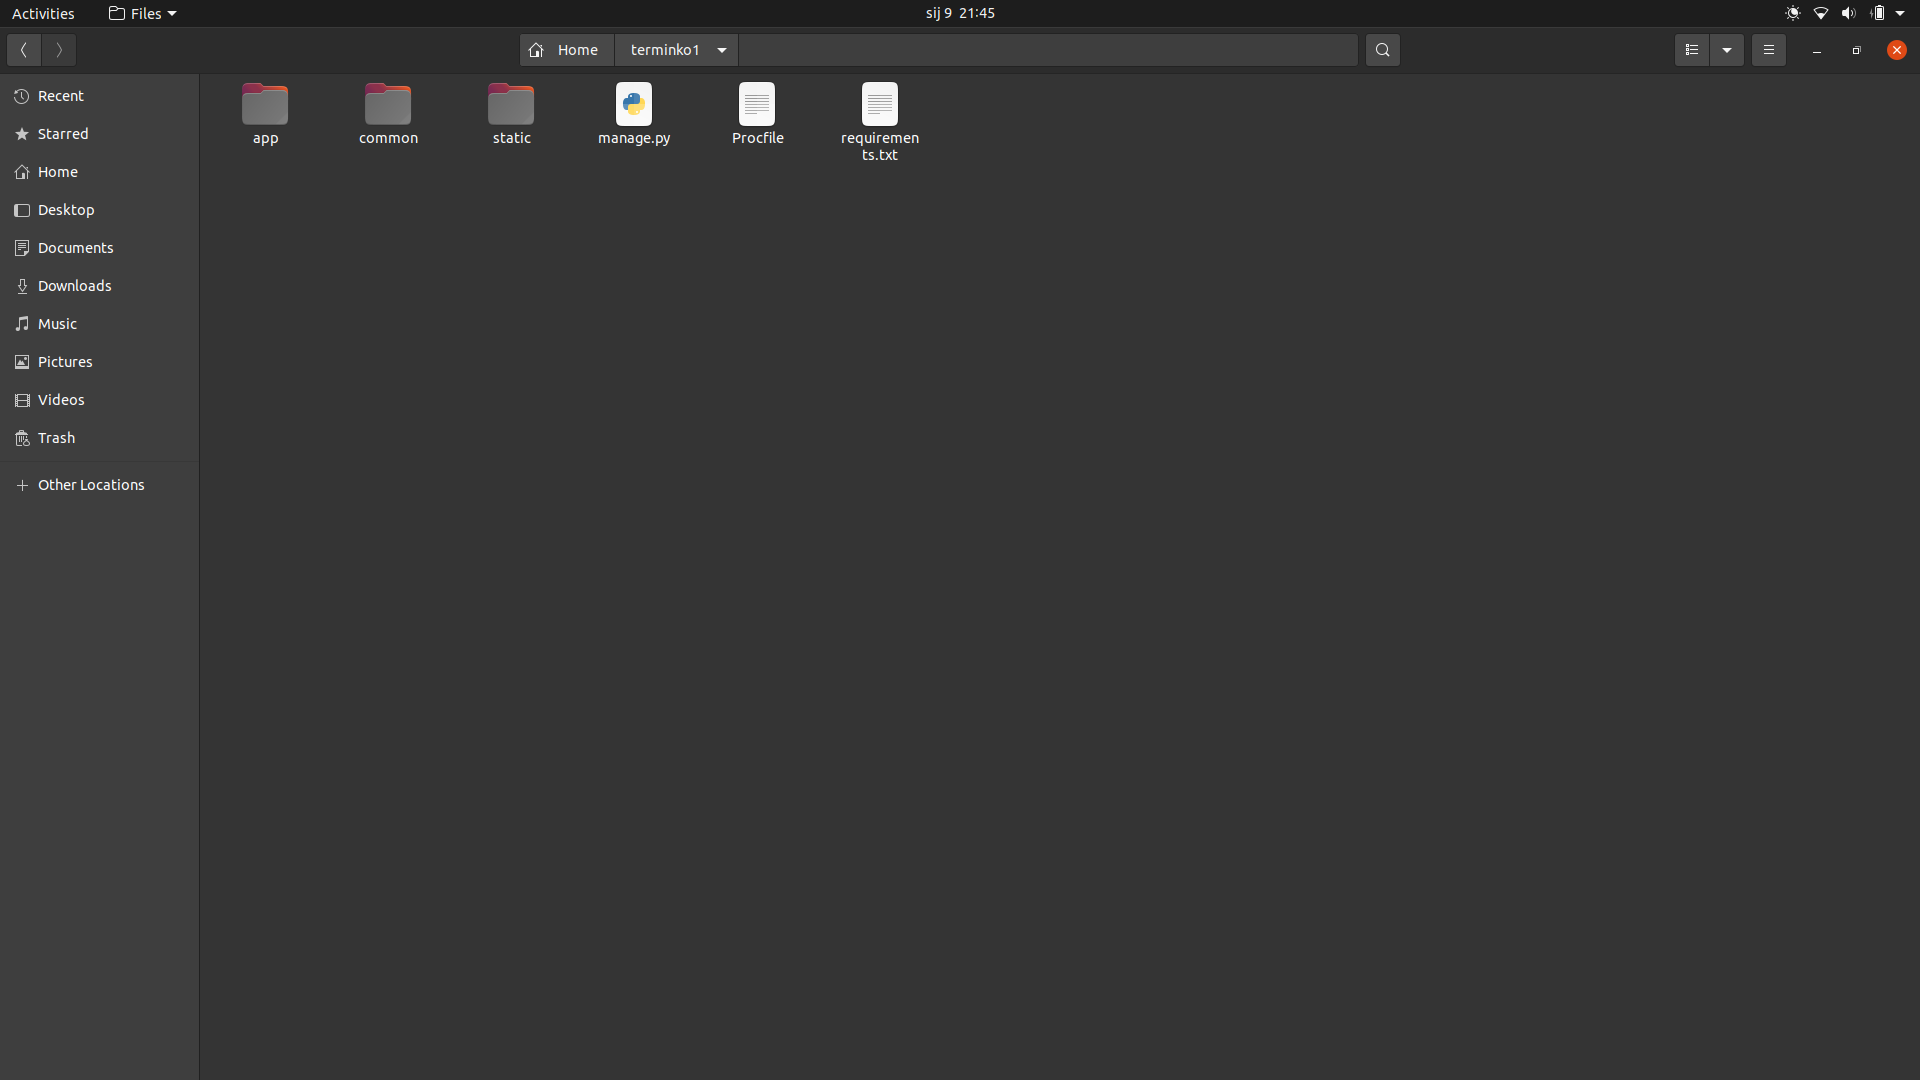
\includegraphics[scale=0.25]{slike/BackendMapa.PNG}
				\caption{Mapa za backend: terminko1}
				\label{fig:promjene}
			\end{figure}
		
			Prvo smo na heroku postavili klijentsku stranu na način da smo prvo napravili aplikaciju terminko. Nakon izrade aplikacije, u odjeljku settings postavili smo konfiguracijske varijable kako je prikazano na slici te smo dodali "buildpack" za Node.js.
			
			\begin{figure}[H]
				\centering
				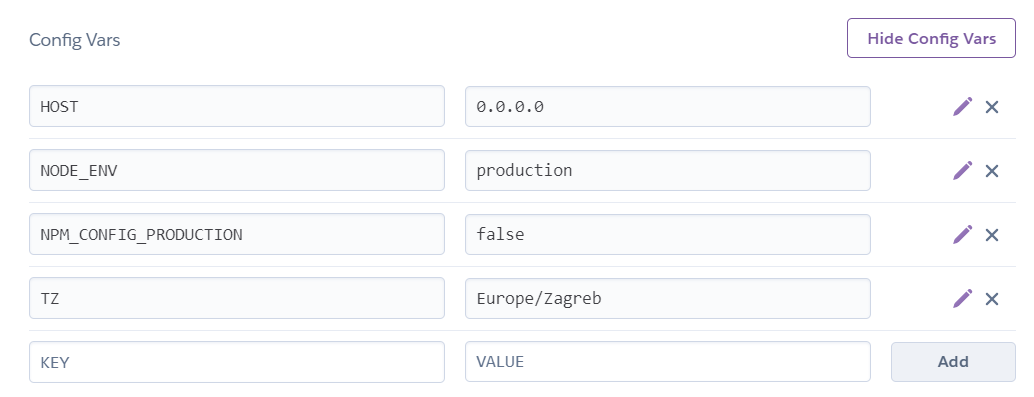
\includegraphics[scale=0.65]{slike/KonfiguracijaFrontend.PNG}
				\caption{Konfiguracija za frontend}
				\label{fig:promjene}
			\end{figure}
		
			\begin{figure}[H]
				\centering
				\includegraphics[scale=0.45]{slike/BuildpackFrontend.PNG}
				\caption{Buildpack za frontend}
				\label{fig:promjene}
			\end{figure}
		
			Na lokalnom smo stroju, u mapu terminko dodali Procfile i u nuxt-config.js dodali novi base-URL za upite na backend
			
			\begin{figure}[H]
				\centering
				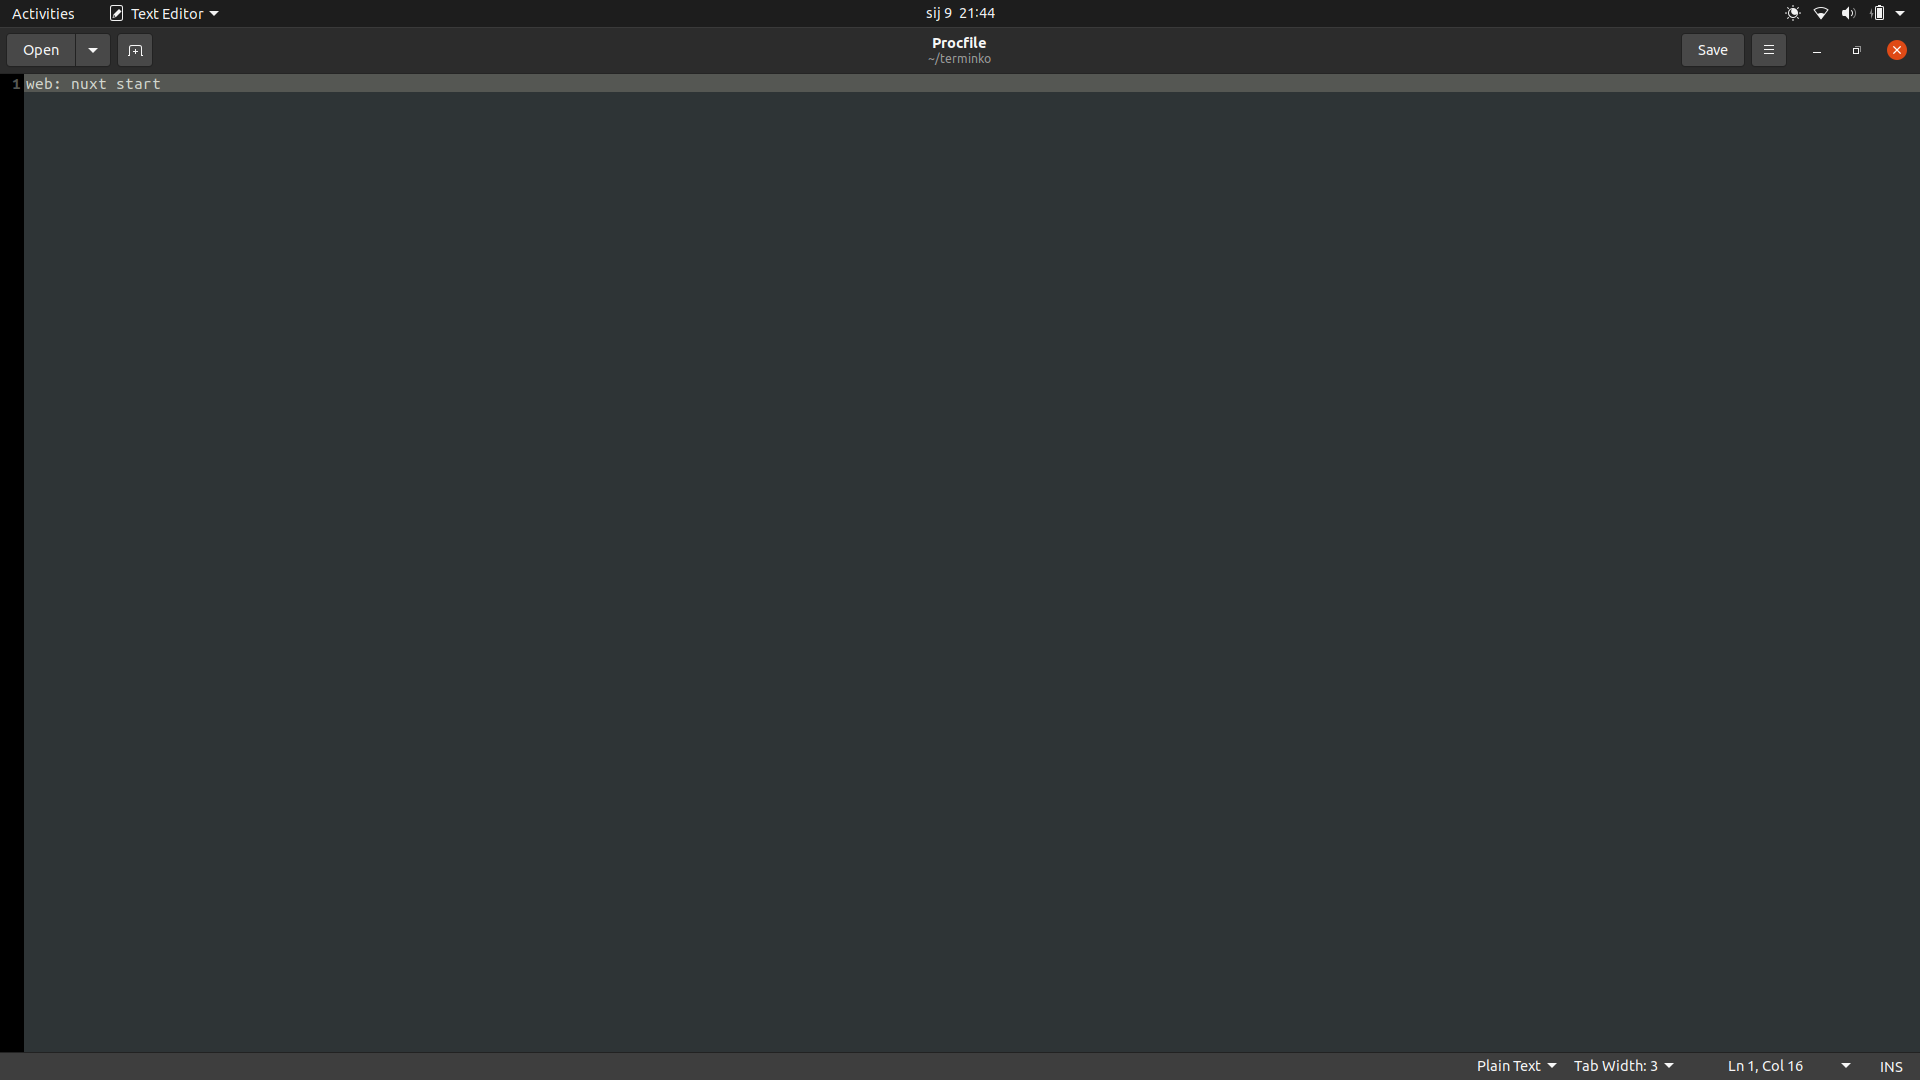
\includegraphics[scale=0.25]{slike/ProcFileFrontend.PNG}
				\caption{Procfile za frontend}
				\label{fig:promjene}
			\end{figure}
			
			\begin{figure}[H]
				\centering
				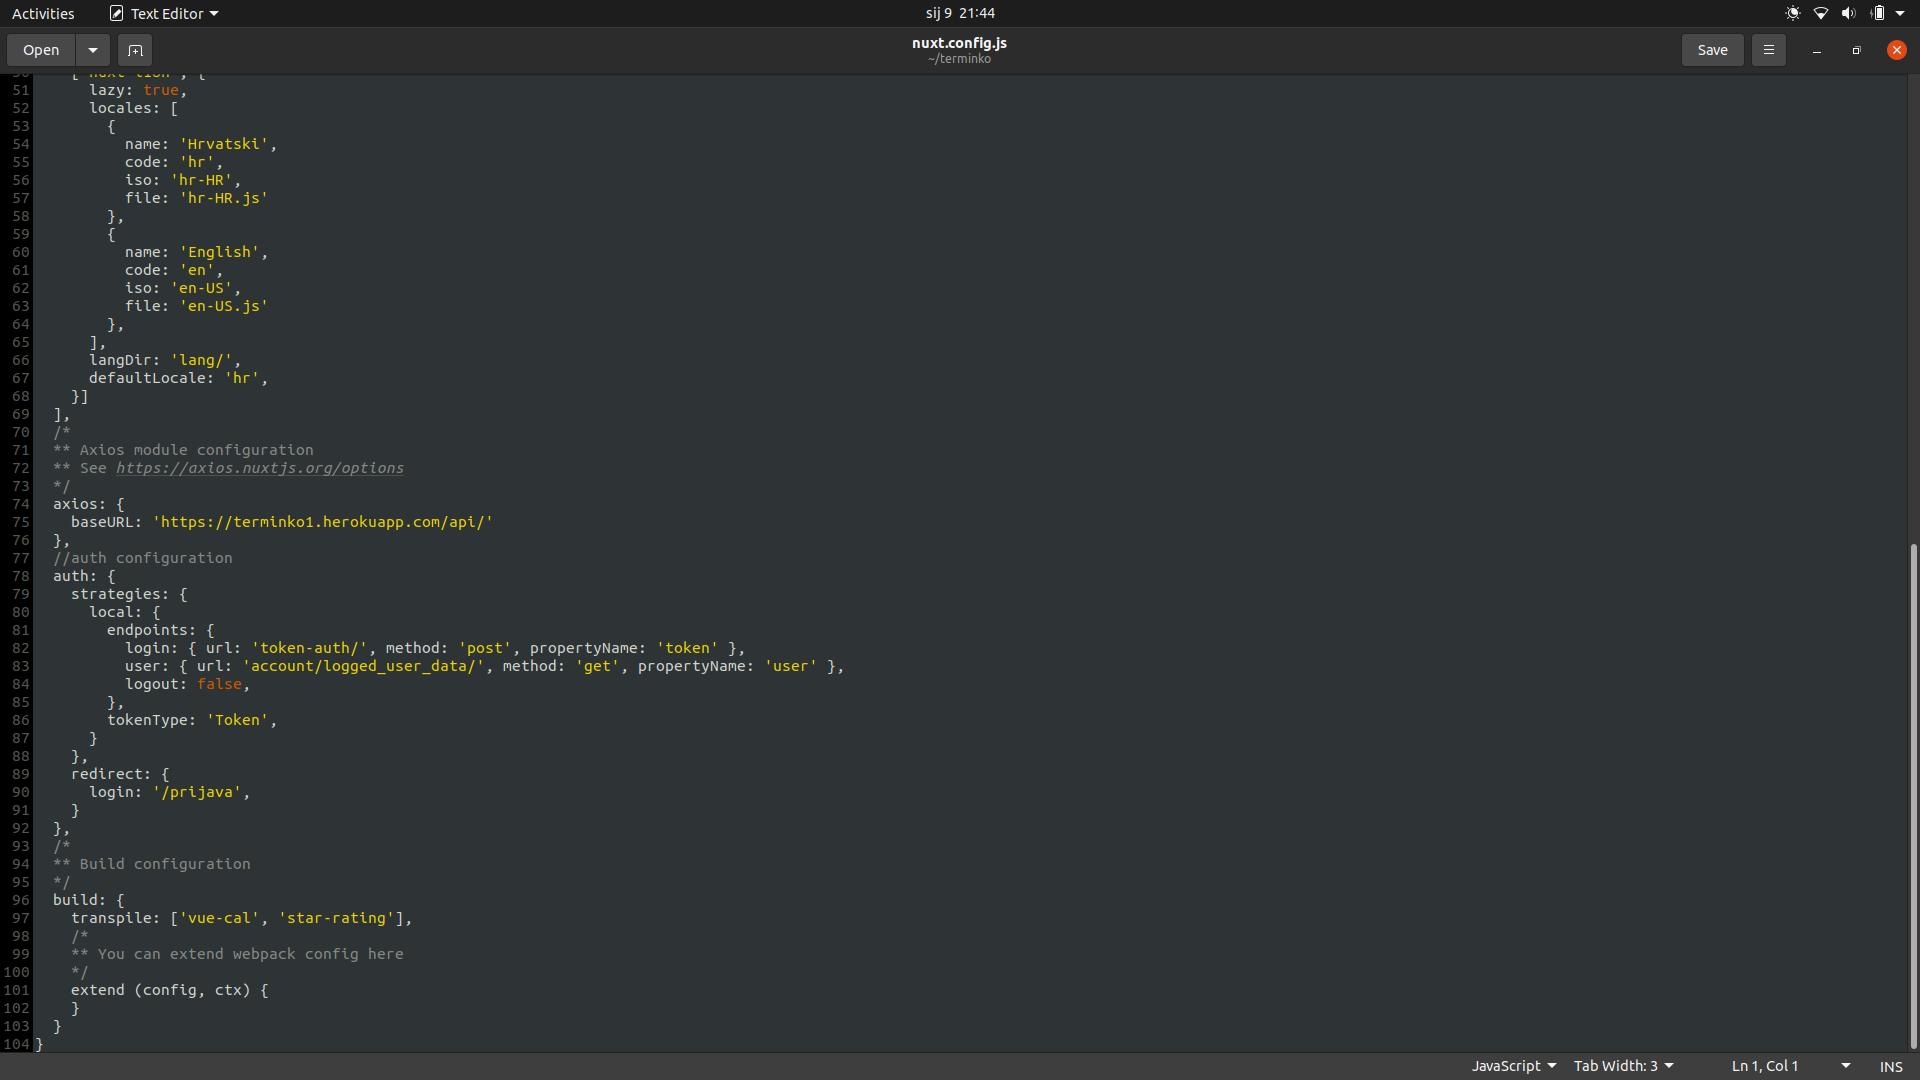
\includegraphics[scale=0.25]{slike/PromjenaFrontend.PNG}
				\caption{Promjena axios base-URL}
				\label{fig:promjene}
			\end{figure}
		
			Nakon toga, još nam je preosalo pozicionirati se u terminko mapu u terminalu, napisati naredbe git init, heroku git:remote -a terminko i git push heroku master. Nakon toga je klijentska strana bila spremna te smo krenuli s poslužiteljskom stranom.
			
			Za poslužiteljsku smo stranu napravili aplikaciju terminko1 na heroku. Na poslužiteljskoj strani nije bilo konfiguracijskih varijabli, dok smo za "buildpack" stavili heroku/python u settings odjeljku. Za razliku od fontenda, na backendu smo na heroku, u tabu resources dodali Heroku Postgres.
			
			\begin{figure}[H]
				\centering
				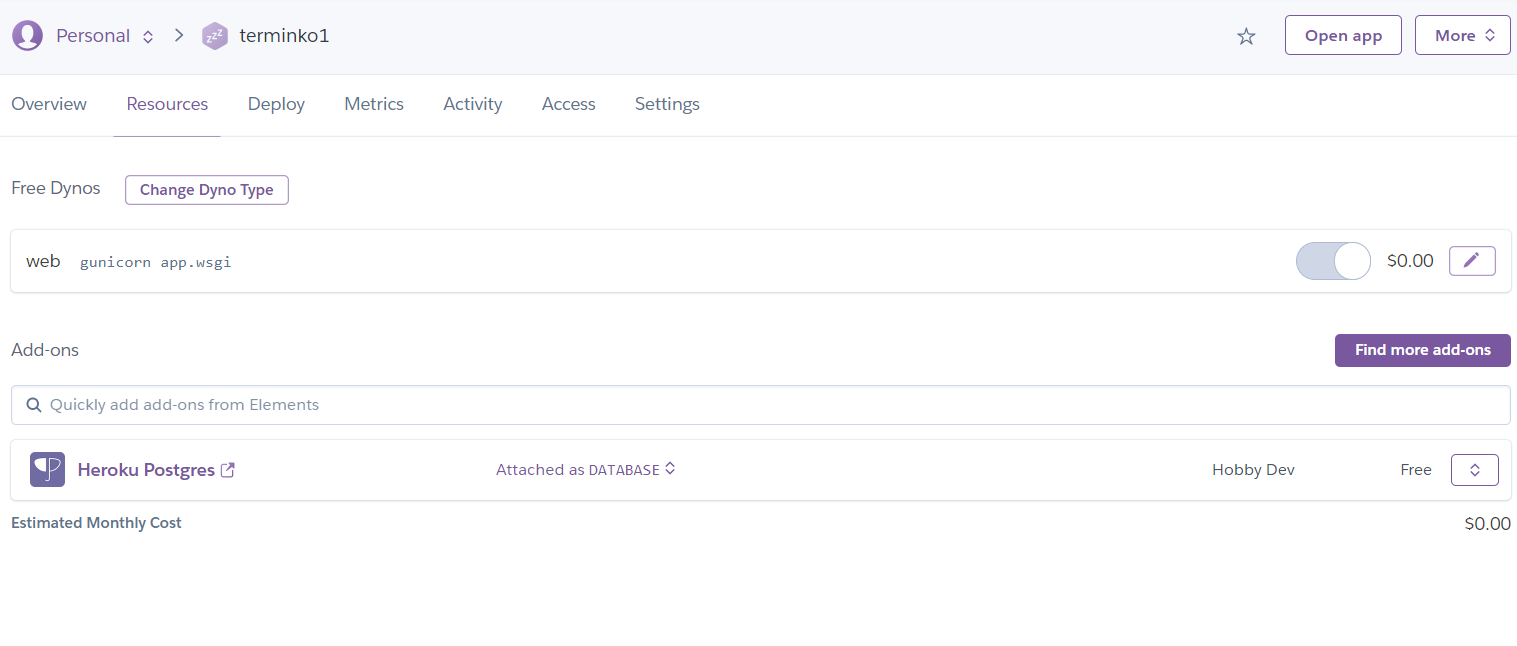
\includegraphics[scale=0.50]{slike/Postgres.PNG}
				\caption{Postavljanje Postgres baze podataka na heroku}
				\label{fig:promjene}
			\end{figure}
		
			Dakako i u mapu terminko1 morali smo dodati Procfile.
			
			\begin{figure}[H]
				\centering
				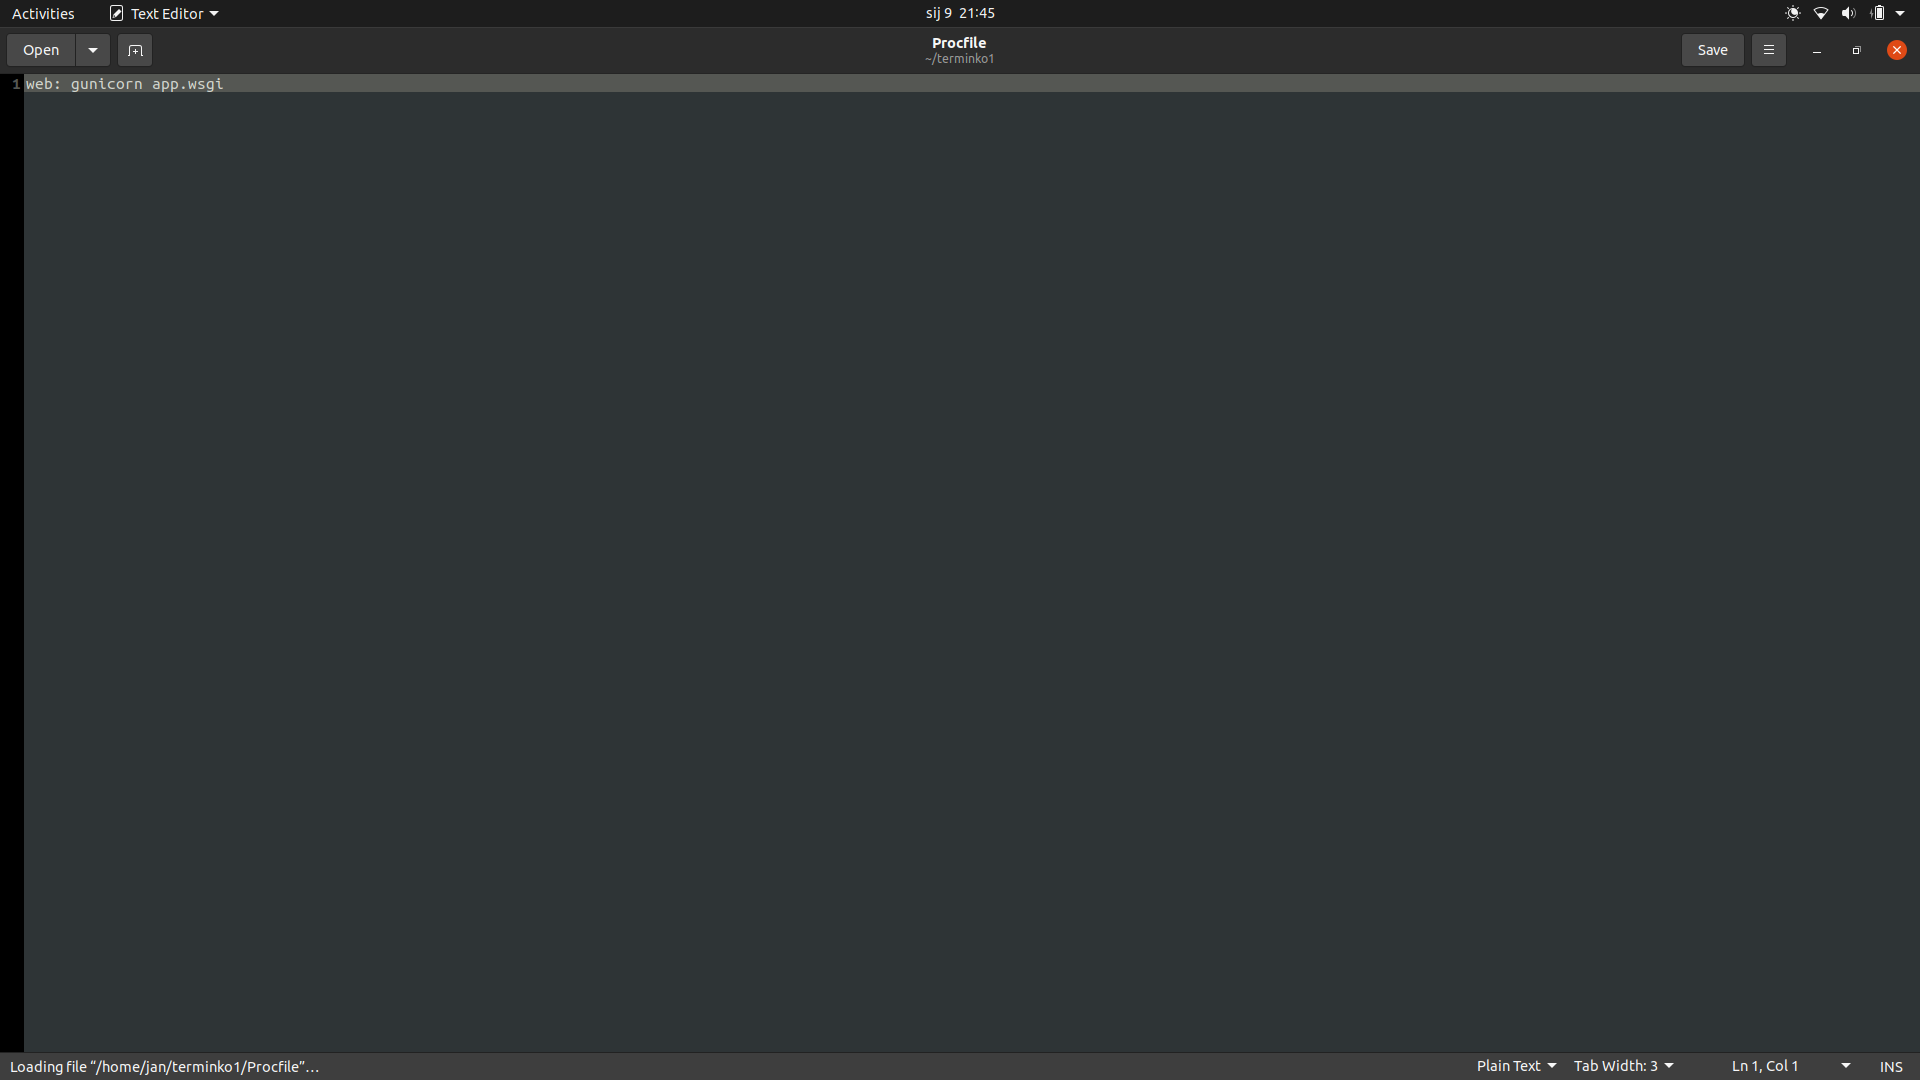
\includegraphics[scale=0.25]{slike/ProcFileBackend.PNG}
				\caption{Procfile na backendu}
				\label{fig:promjene}
			\end{figure}
		
			Nakon toga, dobili smo podatke za prijavu na postgres server koje smo stavili u settings.py datoteku na backendu. U istoj smo datoteci promjenili i CORS origin whitelist, koji označava odalke nas backend može primati zahtjeve, te allowed hosts, koji označava na kojim se poslužiteljima naš backend smije pokretati.
			
			\begin{figure}[H]
				\centering
				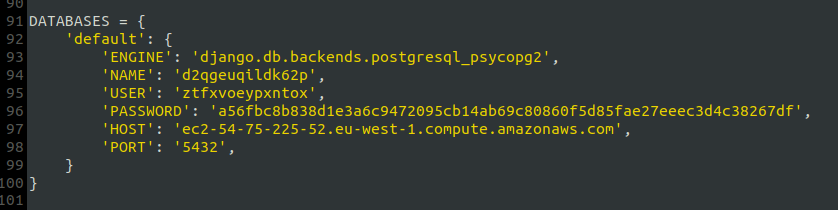
\includegraphics[scale=0.50]{slike/DatabaseData.PNG}
				\caption{Postavljanje Postgres konfiguracije u settings.py}
				\label{fig:promjene}
			\end{figure}
		
			\begin{figure}[H]
				\centering
				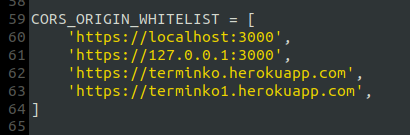
\includegraphics[scale=0.80]{slike/CorsWhitelist.PNG}
				\caption{Postavljanje cors whitelist u settings.py}
				\label{fig:promjene}
			\end{figure}
		
			\begin{figure}[H]
				\centering
				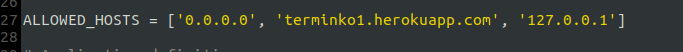
\includegraphics[scale=0.60]{slike/AllowedHosts.PNG}
				\caption{Postavljanje allowed hosts varijable u settings.py}
				\label{fig:promjene}
			\end{figure}
		
			Nakon toga, još nam je preosalo pozicionirati se u terminko1 mapu u terminalu, napisati naredbe git init, heroku git:remote -a terminko1 i git push heroku master. Nakon toga, cijela je aplikacija bila spremna. 
			
			\begin{figure}[H]
				\centering
				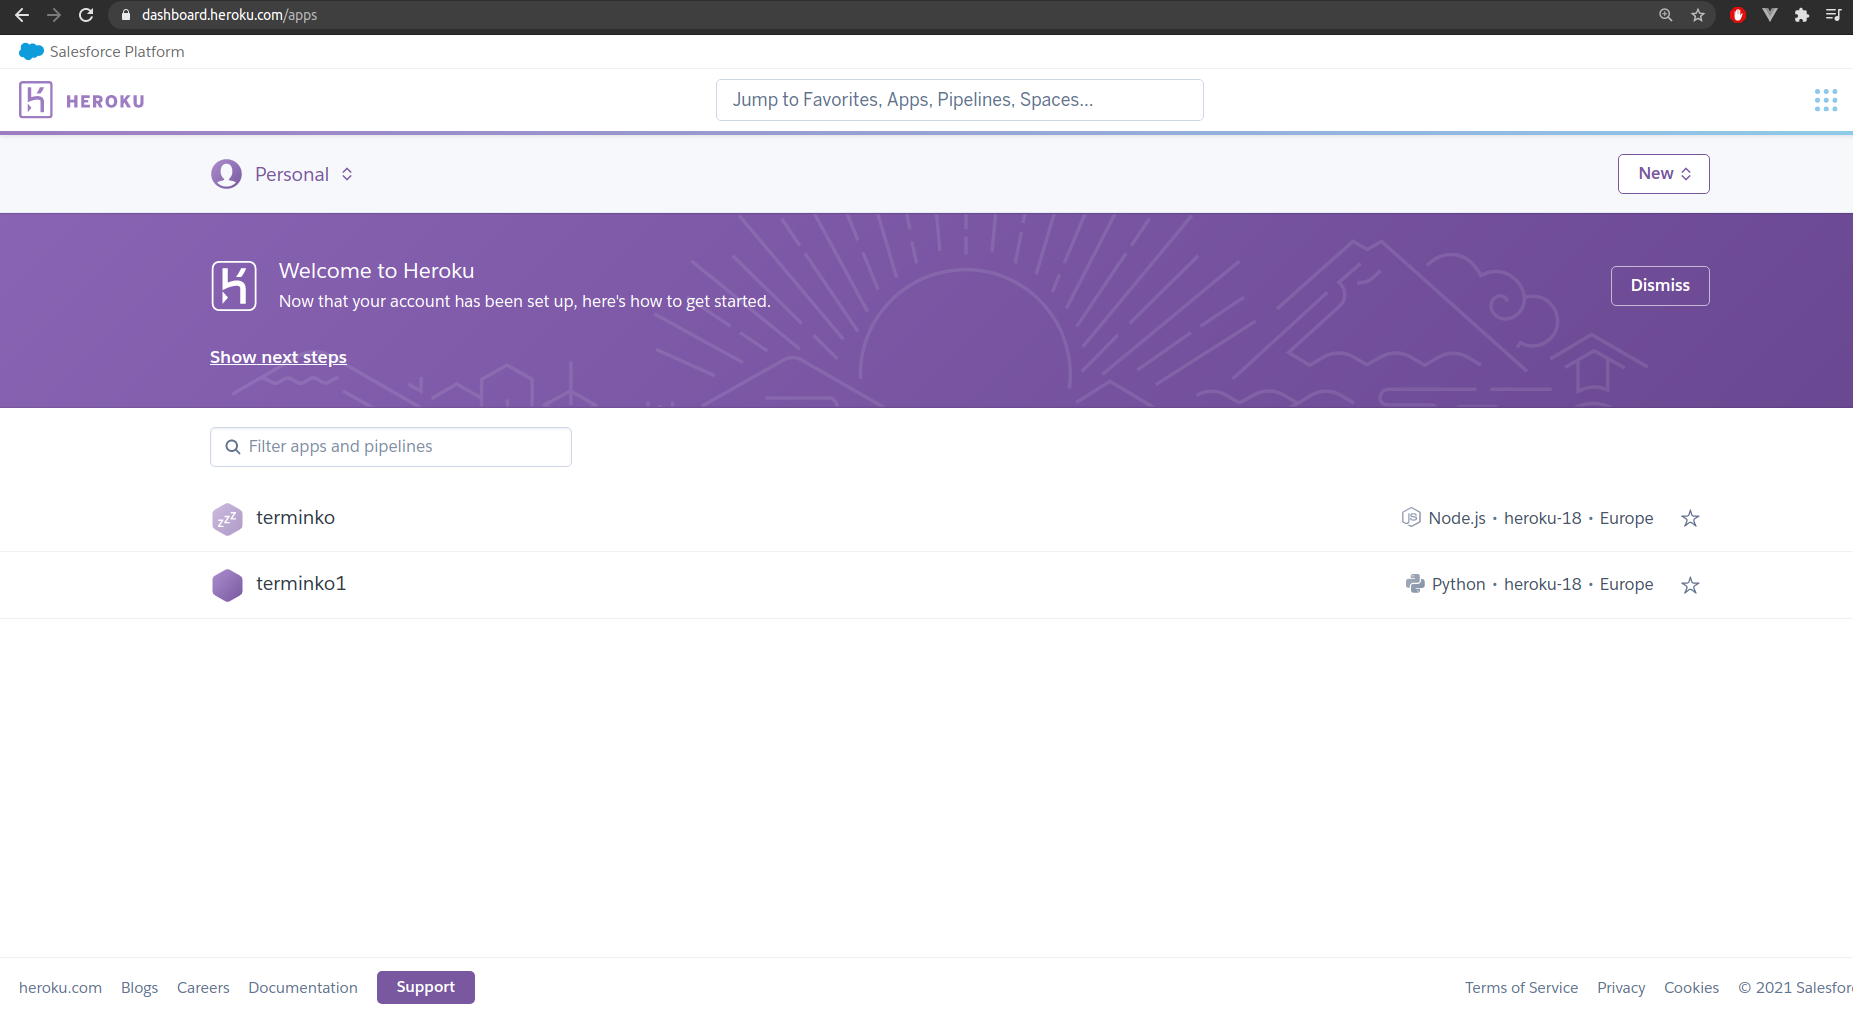
\includegraphics[scale=0.20]{slike/HerokuAplikacije.PNG}
				\caption{Prikaz stanja na heroku po završetku deploya}
				\label{fig:promjene}
			\end{figure}
	\chapter{Zaključak i budući rad}
		\begin{comment}
			content..\textbf{\textit{dio 2. revizije}}\\
			
			\textit{U ovom poglavlju potrebno je napisati osvrt na vrijeme izrade projektnog zadatka, koji su tehnički izazovi prepoznati, jesu li riješeni ili kako bi mogli biti riješeni, koja su znanja stečena pri izradi projekta, koja bi znanja bila posebno potrebna za brže i kvalitetnije ostvarenje projekta i koje bi bile perspektive za nastavak rada u projektnoj grupi.}
			
			\textit{Potrebno je točno popisati funkcionalnosti koje nisu implementirane u ostvarenoj aplikaciji.}.
		\end{comment}
		
		Projekt kojim smo se bavili tijekom semestra bio je izrada web aplikacije 
		za rezerviranje termina u praonici rublja koja bi
		prvenstveno olakšala taj proces studentima, ali i zaposlenicima iste s 
		potencijalom primjene aplikacije i na druge sustave.
		Nakon tromjesečnog
		timskog rada i razvoja aplikacije ostvarili smo zadani cilj. Izvedba projekta
		odvijala se u dvije faze.
		
		U prvoj fazi projekta naglasak je bio na okupljanju tima, 
		njegovom upoznavanju, analiziranju sposobnosti i okvirnoj raspodjeli
		budućih poslova. Isto tako, većina se vremena posvetila
		osmišljavanju funkcionalnosti, analiziranju zahtjeva te 
		dokumentiranju istih. Detaljna dokumentacija u koju smo uložili mnogo truda
		i vremena bila je izvrstan temelj za drugu fazu izvedbe projekta. 
		Funkcionalni zahtjevi, obrasci uporabe, sekvencijski dijagrami, model baze
		podataka i dijagram razreda bili su veoma koristan alat kojim smo rješavali
		implementacijske nedoumice. 
		
		Druga faza projekta sadržavala je u najvećem dijelu programiranje i
		implementaciju dokumentirane web aplikacije. Ta faza zahtjevala je 
		poseban samostalni angažman članova tima koji se dotada nisu susreli
		s tehnologijama koje smo odlučili koristiti, ali i angažman 
		članova tima koji su s tim tehnologijama bili upoznati kako bi
		pomogli kolegama da ih što uspješnije savladaju. Tijekom tog vremena
		vladao je visok intenzitet rada i odlična timska kohezija. Isto tako, 
		bilo je potrebno napisati preostalu dokumentaciju i izraditi UML dijagrame.
		
		Pri izradi projekta mnogo toga smo naučili, od korištenja novih tehnologija,
		alata, usavršavanja programskih jezika, izrade dokumentacije
		do važnosti i koristi koje nam pruža timski rad, kolegijalni i dobri
		timski odnosi, organiziran i marljiv voditelj tima koji koordinira
		svim aktivnostima, ali i vrijedni članovi
		koji prihvaćaju sugestiju te teže napretku u svakom smislu.
		Također smo naučili vrijednost kontinuiranog rada koji nam je olakšao
		da sve zadatke obavimo na vrijeme i bez panike. Izuzetno smo zadovoljni
		izrađenom web aplikacijom, ali smo isto tako svjesni da ima dosta mjesta
		za napredak i usavršavanje iste. Jedna od mogućnosti bi bila proširenje 
		aplikacije za hotelske sustave ili samoposlužne praonice, ali i izrada mobilne 
		aplikacije.
		\eject 
	\chapter*{Popis literature}
		\addcontentsline{toc}{chapter}{Popis literature}
	 	
 		\textbf{\textit{Kontinuirano osvježavanje}}
	
		\textit{Popisati sve reference i literaturu koja je pomogla pri ostvarivanju projekta.}
		
		
		\begin{enumerate}
			
			
			\item  Programsko inženjerstvo, FER ZEMRIS, \url{http://www.fer.hr/predmet/proinz}
			
			\item  Astah Community, \url{http://astah.net/editions/uml-new}
			
			\item  Nuxt documentation, \url{https://nuxtjs.org/}
			
			\item  Django documentation, \url{https://docs.djangoproject.com/en/3.1/}
		\end{enumerate}
		
		 
	
	
	\begingroup
	\renewcommand*\listfigurename{Indeks slika i dijagrama}
	%\renewcommand*\listtablename{Indeks tablica}
	%\let\clearpage\relax
	\listoffigures
	%\vspace{10mm}
	%\listoftables
	\endgroup
	\addcontentsline{toc}{chapter}{Indeks slika i dijagrama}


	
	\eject 
		
	\chapter*{Dodatak: Prikaz aktivnosti grupe}
\addcontentsline{toc}{chapter}{Dodatak: Prikaz aktivnosti grupe}

\section*{Dnevnik sastajanja}

\textbf{\textit{Kontinuirano osvježavanje}}\\

\textit{U ovom dijelu potrebno je redovito osvježavati dnevnik sastajanja prema predlošku.}

\begin{packed_enum}
	\item  sastanak
	
	\item[] \begin{packed_item}
		\item Datum: 2. listopada 2020.
		\item Prisustvovali: I. Joskić, D. Grgić, B. Spiegl, D. Šmigovec, M. Dragošević, L. Inkret, J. Grgić
		\item Teme sastanka:
		\begin{packed_item}
			\item  smišljanje teme za projekt
		\end{packed_item}
	\end{packed_item}
	
	\item  sastanak
	\item[] \begin{packed_item}
		\item Datum: 15. listopada 2020.
		\item Prisustvovali: I. Joskić, D. Grgić, B. Spiegl, D. Šmigovec, M. Dragošević, L. Inkret, J. Grgić
		\item Teme sastanka:
		\begin{packed_item}
			\item  rasprava o funkcionalnostima sustava
			\item  rasprava o bazi podataka
		\end{packed_item}
	\end{packed_item}

	\item  sastanak
	\item[] \begin{packed_item}
		\item Datum: 26. listopada 2020.
		\item Prisustvovali: I. Joskić, D. Grgić, B. Spiegl, D. Šmigovec, M. Dragošević, L. Inkret, J. Grgić
		\item Teme sastanka:
		\begin{packed_item}
			\item  rasprava o funkcionalnostima sustava
			\item  rasprava o bazi podataka
			\item  promijene i dodaci u do sad napisanom dokumentu vezane za bazu podataka, funkcionalne i nefunkcionalne zahtjeve i obrazaca uporabe
		\end{packed_item}
	\end{packed_item}

	\item  sastanak
	\item[] \begin{packed_item}
		\item Datum: 29. listopada 2020.
		\item Prisustvovali: I. Joskić, D. Grgić, B. Spiegl, D. Šmigovec, M. Dragošević, J. Grgić
		\item Teme sastanka:
		\begin{packed_item}
			\item  rasprava bazi podataka
			\item  rasprava o dijagramima obrasca uporabe
			\item  prijedlozi za dodatke i promijene u dokumentu
		\end{packed_item}
	\end{packed_item}
	
	%
	
\end{packed_enum}

\eject
\section*{Tablica aktivnosti}

\textbf{\textit{Kontinuirano osvježavanje}}\\

\textit{Napomena: Doprinose u aktivnostima treba navesti u satima po članovima grupe po aktivnosti.}



\begin{longtabu} to \textwidth {|X[7, l]|X[1, c]|X[1, c]|X[1, c]|X[1, c]|X[1, c]|X[1, c]|X[1, c]|}
	
	\cline{2-8} \multicolumn{1}{c|}{\textbf{}} &     \multicolumn{1}{c|}{\rotatebox{90}{\textbf{Jan Grgić }}} & \multicolumn{1}{c|}{\rotatebox{90}{\textbf{Dunja Šmigovec }}} &	\multicolumn{1}{c|}{\rotatebox{90}{\textbf{Marija Dragošević }}} &	\multicolumn{1}{c|}{\rotatebox{90}{\textbf{Bernard Spiegl }}} &
	\multicolumn{1}{c|}{\rotatebox{90}{\textbf{Dino Grgić }}} &
	\multicolumn{1}{c|}{\rotatebox{90}{\textbf{Ivan Joskić }}} &	\multicolumn{1}{c|}{\rotatebox{90}{\textbf{Leonard Inkret }}} \\ \hline 
	\endfirsthead
	
	
	\cline{2-8} \multicolumn{1}{c|}{\textbf{}} &     \multicolumn{1}{c|}{\rotatebox{90}{\textbf{Jan Grgić }}} & \multicolumn{1}{c|}{\rotatebox{90}{\textbf{Dunja Šmigovec }}} &	\multicolumn{1}{c|}{\rotatebox{90}{\textbf{Marija Dragošević }}} &
	\multicolumn{1}{c|}{\rotatebox{90}{\textbf{Bernard Spiegl }}} &	\multicolumn{1}{c|}{\rotatebox{90}{\textbf{Dino Grgić }}} &
	\multicolumn{1}{c|}{\rotatebox{90}{\textbf{Ivan Joskić }}} &	\multicolumn{1}{c|}{\rotatebox{90}{\textbf{Leonard Inkret }}} \\ \hline 
	\endhead
	
	
	\endfoot
	
	%aaa
	\endlastfoot
	Upravljanje projektom 		& 4 &  &  &  &  &  & \\ \hline
	Opis projektnog zadatka 	& 5 & 2 & 1:30 & 2 & 2 & 2 & \\ \hline	
	Funkcionalni zahtjevi       & 1 & 0:30 & 1 & 1 & 0:30 & 1:30 &  \\ \hline
	Opis pojedinih obrazaca 	& 3:30 & 1 & 3 & 3 & 1 & 5 &  \\ \hline
	Dijagram obrazaca 			& 1:30 & 1 & 1 & 2:30 & 1 & 1 &  \\ \hline
	Sekvencijski dijagrami 		&  & 3 &  &  &  & 4 &  \\ \hline
	Opis ostalih zahtjeva 		&  &  &  &  & 1 &  &  \\ \hline
	Arhitektura i dizajn sustava	 &  &  &  &  &  4  &  & \\ \hline
	Baza podataka				& 1:30 & 6:30 & 0:30 & 0:30 & 0:30 & 0:30 &   \\ \hline
	Dijagram razreda 			&  &  &  &   & 4 &  &   \\ \hline
	Dijagram stanja				&  &  &  &  &  &  &  \\ \hline
	Dijagram aktivnosti 		&  &  &  &  &  &  &  \\ \hline
	Dijagram komponenti			&  &  &  &  &  &  &  \\ \hline
	Korištene tehnologije i alati 		&  &  &  &  &  &  &  \\ \hline
	Ispitivanje programskog rješenja 	&  &  &  &  &  &  &  \\ \hline
	Dijagram razmještaja			&  &  &  &  &  &  &  \\ \hline
	Upute za puštanje u pogon 		&  &  &  &  &  &  &  \\ \hline 
	Dnevnik sastajanja 			& 0:30 &  &  &  &  &  &  \\ \hline
	Zaključak i budući rad 		&  &  &  &  &  &  &  \\  \hline
	Popis literature 			&  &  &  &  &  &  &  \\  \hline
	&  &  &  &  &  &  &  \\ \hline \hline
	\textit{izrada frontenda} 				& 12 &  & 3 &  & 0:30  &  &  \\ \hline 
	\textit{izrada backenda} 		 		& 16 &  &  &  & 1  &  & \\ \hline 
	\textit{spajanje frontenda s back endom} 							& 2 &  &  &  & 0:30  &  &  \\ \hline
	&  &  &  &  &  &  &\\  \hline
	
	
\end{longtabu}


\eject
\section*{Dijagrami pregleda promjena}

\textbf{\textit{dio 2. revizije}}\\

\textit{Prenijeti dijagram pregleda promjena nad datotekama projekta. Potrebno je na kraju projekta generirane grafove s gitlaba prenijeti u ovo poglavlje dokumentacije. Dijagrami za vlastiti projekt se mogu preuzeti s gitlab.com stranice, u izborniku Repository, pritiskom na stavku Contributors.}




\end{document} %naredbe i tekst nakon ove naredbe ne ulaze u izgrađen dokument 


